% !Mode:: "TeX:UTF-8"
\documentclass[type=doctor, openany, pifootnote]{shuthesis}
% 选项：
%  type=[master|doctor],            % 必选
%  secret,                          % 可选 (如果论文需要保密，这一项需要打开)
%  pifootnote,                      % 可选（建议打开）
%  openany|openright,               % 可选 (章首页是右开还是任意开，默认是右开)
%  nocolor                          % 提交最终版本时请打开此选项
\usepackage{pdfpages}
\usepackage{shuthesis}
\usepackage{gbt7714}
\usepackage{ctex}
\usepackage{tikz}
\usepackage{graphicx}
\usetikzlibrary{
    positioning,      % 用于 node distance 和 relative positioning
    arrows.meta,      % 用于箭头样式
    shapes.geometric, % 几何形状
    calc,             % 坐标计算
    fit,              % 节点拟合
    backgrounds       % 背景层
}
\bibliographystyle{gbt7714-numerical}
\citestyle{super}                   % 默认引用为角标格式，正文格式为\citestyle{numbers}


\graphicspath{{figures/}}

% 中文章节序号
\ctexset{
  chapter = {
    name = {第,章},
    number = \chinese{chapter}
  }
}
% 中文正文字体：
\setCJKmainfont[
    ExternalLocation=./fonts/,
    AutoFakeBold=true,
    ItalicFont=SimKai.ttf,
    BoldItalicFont=SimKai.ttf
]{SimSun.ttf}
% 中文 sansfont, 主要出现在 section 的标题中：
\setCJKsansfont[
    ExternalLocation=./fonts/,
    AutoFakeBold=true
]{SimHei.ttf}


% 英文正文的字体：
\setmainfont[
    BoldFont=Times New Roman Bold,
    ItalicFont=Times New Roman Italic,
    BoldItalicFont=Times New Roman Bold Italic
]{Times New Roman}
% 英文的 sansfont 主要出现在 section 的标题中 (这里就把 Regular 直接设置为了 TimesNewRoman-Bold):
\setsansfont[
    BoldFont=Times New Roman Bold,
    ItalicFont=Times New Roman Bold Italic,
    BoldItalicFont=Times New Roman Bold Italic
]{Times New Roman Bold}
% 英文的 monofont 主要出现在代码中 (\texttt), 可以根据自己的喜好调整：
\setmonofont[
    BoldFont=Times New Roman Bold,
    ItalicFont=Times New Roman Italic,
    BoldItalicFont=Times New Roman Bold Italic
]{Times New Roman}


% 下面是论文相关信息的填写：
% 论文题目：
\newcommand{\iTitle}{基于Transformer的点云补全模型与三维重建算法研究}
% 学院：
\newcommand{\iSchool}{计算机工程与科学学院}
% 专业：
\newcommand{\iMajor}{计算机科学与技术}
% 学号：
\newcommand{\iStudentNumber}{22122787}
% 学生姓名：
\newcommand{\iStudentName}{张嘉翊}
% 指导老师：
\newcommand{\iSupervisorName}{张景峤}
% 起讫时间：
\newcommand{\iThesisTime}{2026 年 3 月 2 日至 2026 年 5 月 29 日}

\begin{document}
\include{contents/cover}
\include{contents/declaration}

% 如果需要直接覆盖封面和原创性声明，请将下面一行取消注释，并注释上面两行。
% \includepdf[pages={1,2}]{cover.pdf}

\frontmatter
\newpage

\setcounter{page}{1} % skip the content page

{
% \cleardoublepage% Move to first page of new chapter
\let\clearpage\relax% Don't allow page break
\chapter*{摘\ 要}
}
\addcontentsline{toc}{chapter}{摘\ 要}

三维点云数据可精准表达物体空间几何结构，在自动驾驶、机器人环境感知、增强现实等领域得到广泛应用。受采集设备性能、物体遮挡、视点受限等因素影响，实际获取的点云往往存在稀疏残缺问题，严重制约后续三维处理任务的精度与鲁棒性。传统点云补全方法在复杂结构与大面积缺失场景下效果有限，早期深度学习方法易出现局部细节丢失问题，已有的基于Transformer架构的方法虽然可以在补全任务中兼顾点云全局结构与局部细节，但难以保证补全后点云全局密度的均衡分布。本文针对以上问题，开展基于Transformer的点云补全与三维重建算法研究，基于Coarse-to-fine渐进式生成策略，引入自适应查询生成机制与基于损失函数的密度感知强化，提高了模型的点云补全性能与密度感知能力。实验基于ShapeNet等公开数据集开展，结果表明本算法在补全精度上优于主流基准方法，可为三维视觉相关应用提供有效的算法支撑。

\vspace{8mm}
\textbf{关键词}: 点云补全, Transformer, 三维重建

\newpage
{
% \cleardoublepage% Move to first page of new chapter
\let\clearpage\relax% Don't allow page break
\chapter*{ABSTRACT}
}
\addcontentsline{toc}{chapter}{ABSTRACT}

Three-dimensional point cloud data can accurately represent the spatial geometric structure of objects, and has been widely applied in autonomous driving, robotic environmental perception, augmented reality, and other fields. Due to factors such as the performance limitations of acquisition equipment, object occlusion, and restricted viewpoints, the acquired point clouds often suffer from sparsity and incompleteness, which severely constrains the accuracy and robustness of subsequent 3D processing tasks. Traditional point cloud completion methods exhibit limited effectiveness in scenarios with complex structures and large-area missing regions. Early deep learning-based approaches are prone to losing local details. Although existing Transformer-based methods can balance global structure and local details in completion tasks, they struggle to ensure the uniform distribution of global point density in the completed point clouds. To address these issues, this paper conducts research on Transformer-based point cloud completion and 3D reconstruction algorithms. Based on a Coarse-to-Fine progressive generation strategy, an adaptive query generation mechanism and density-aware reinforcement through loss function design are introduced, which improve the model's point cloud completion performance and density-aware capability. Experiments are conducted on public datasets such as ShapeNet. The results demonstrate that the proposed algorithm outperforms mainstream baseline methods in completion accuracy, providing effective algorithmic support for 3D vision-related applications.

\vspace{8mm}

\textbf{Keywords}: Point Cloud Completion, Transformer, 3D Reconstruction



{
    \hypersetup{linkcolor=black}
    \tableofcontents
    \thispagestyle{shu@nopagefoot}
}


\mainmatter
% !Mode:: "TeX:UTF-8"
\chapter{绪论}
\label{cha:intro}

\section{研究背景与意义}

\subsection{三维点云数据应用场景}
三维点云是三维空间中离散采样点的集合，能够直接、精准地还原现实世界中物体与场景的三维几何结构，是当前三维视觉领域最核心的数据表示形式之一。与二维图像相比，点云数据不受光照、视角变化带来的尺度歧义影响，能够直接提供物体的三维空间坐标信息，因此在众多工业与科研领域得到了广泛的应用。

在自动驾驶领域，激光雷达（LiDAR）采集的点云数据是环境感知系统的核心数据源，其能够在复杂光照与天气条件下，提供高精度的三维空间位置信息，是自动驾驶车辆实现障碍物检测、可通行区域分割、实时定位与地图构建（SLAM）的关键基础\cite{zhai2023improved}。通过对车辆周围环境的点云数据进行处理，自动驾驶系统能够准确识别被遮挡的车辆、行人等交通参与者，为路径规划与避障决策提供可靠的环境信息，直接决定了自动驾驶系统的安全性与可靠性。

在工业逆向工程与质量检测领域，通过三维扫描设备获取实体零件的点云数据，能够快速重建出零件的高精度三维数字模型，实现产品的数字化设计、逆向仿制与缺陷检测。对于航空航天、汽车制造等高端制造领域，复杂曲面零件的加工精度要求极高，通过对加工后的零件进行点云扫描，与设计的标准模型进行比对，能够快速、精准地检测出加工误差，大幅提升产品质量检测的效率与精度，缩短产品的研发与生产周期。

在增强现实（AR）与虚拟现实（VR）领域，点云数据能够真实还原现实场景的三维结构，为虚拟物体与现实场景的精准融合提供空间基准，提升沉浸式交互体验。通过对现实场景进行三维点云扫描，能够快速构建出场景的高精度三维数字孪生模型，实现虚拟内容与现实场景的几何匹配，让虚拟物体能够与现实环境产生真实的物理交互，广泛应用于数字文旅、虚拟直播、工业远程运维等场景。

在智慧农业领域，通过深度相机获取的作物与果实点云数据，可实现果实的精准定位、长势监测与产量预估，辅助采摘机器人克服枝叶遮挡带来的感知难题，提升自动化作业的精度与效率\cite{zhai2023improved}。针对农业场景中果实被枝叶大面积遮挡的问题，通过点云补全技术恢复果实的完整几何结构，能够让采摘机器人准确获取果实的位置与形状信息，大幅提升采摘的成功率，推动农业生产的自动化与智能化发展。

\subsection{点云数据残缺问题与挑战}
在实际的工程应用中，三维点云数据的获取主要依赖激光雷达、RGB-D相机、结构光三维扫描仪等设备，受限于设备硬件性能、采集环境与物体自身特性，原始采集得到的点云数据往往无法完整还原物体的全部几何结构，普遍存在稀疏、非均匀、残缺的问题\cite{yu2021pointr}，这也是制约后续三维处理任务精度的核心瓶颈。

采集设备的硬件性能是导致点云质量下降的基础因素。激光雷达的角分辨率直接决定了点云的采样密度，对于远距离的物体，采集到的点云往往较为稀疏，无法还原物体的精细几何结构；同时激光雷达的测量范围有限，对于超出量程的区域，无法获取有效的深度信息。RGB-D相机通过红外结构光或飞行时间原理测量深度，对于高反光、透明材质的物体表面，深度测量会出现严重的噪声与缺失；同时受限于相机的视场角，单张深度图像只能覆盖有限的场景范围，无法获取完整的环境信息。结构光扫描仪虽然能够获取高精度的稠密点云，但其对采集环境的光照条件要求较高，同时对于表面纹理单一的物体，容易出现匹配失效，导致点云出现大面积缺失。

物体自身的遮挡效应是导致点云残缺的最核心因素。在点云采集过程中，物体的自身结构、场景中的其他物体都会对采集视点形成遮挡，被遮挡的区域无法被扫描设备捕捉，从而形成大面积的点云缺失\cite{yu2021pointr}。例如在自动驾驶场景中，前方的大型车辆会遮挡后方的小型车辆与行人，导致激光雷达无法获取被遮挡目标的点云数据；在工业零件扫描过程中，零件的复杂内腔、凹槽结构会形成自遮挡，无法被外部的扫描设备捕捉到完整的几何结构。这种遮挡导致的点云缺失，往往会破坏物体的拓扑结构，导致后续的特征提取与处理出现严重的误差。

采集视点的单一性同样会导致点云数据的不完整。单视点采集只能获取物体朝向相机一侧的表面信息，无法获取物体背面、侧面与内部的几何结构，形成大规模的缺失区域。虽然可以通过多视点采集与点云配准，获取物体更完整的点云数据，但在很多实际场景中，受限于采集环境与操作空间，无法实现多视点的环绕采集，只能获取单视点的残缺点云数据。例如在自动驾驶场景中，车辆只能获取自身行驶方向上的环境点云，无法对周围环境进行全视角的环绕扫描；在逆向工程中，对于大型的工业设备，无法实现无死角的多视点采集，只能获取有限视角下的点云数据。

上述因素导致实际获取的原始点云数据，普遍呈现出稀疏、非均匀、不完整的特性，这种数据缺陷不仅破坏了物体原本的几何拓扑结构，还会直接导致后续的目标检测、语义分割、点云配准、三维重建等任务出现严重的精度下降，甚至无法完成正常的处理流程\cite{yan2022shapeformer}。例如在三维重建任务中，残缺的点云会导致重建的表面出现大量的孔洞，无法生成完整的三维网格模型；在目标检测任务中，残缺的点云会导致网络无法准确提取目标的几何特征，出现漏检、误检等问题。因此，如何从残缺的点云数据中，恢复出物体完整的三维几何结构，是三维视觉领域亟待解决的基础性问题。

\subsection{点云补全与三维重建研究价值}
点云补全（Point Cloud Completion）作为三维视觉领域的一项基础性任务，其核心目标是从残缺的输入点云中，推断并恢复出物体完整的三维几何形状，生成稠密、均匀、完整的点云数据。高质量的点云补全算法，能够有效解决实际采集过程中点云残缺的问题，为后续的三维处理任务提供高质量的完整点云数据，因此具备重要的理论意义与实际应用价值。

在理论研究层面，点云补全任务面临着诸多核心的理论挑战，其研究能够推动三维视觉领域相关理论的发展。点云数据的无序性、稀疏性与不规则性，给特征提取与几何建模带来了极大的难度；而当输入点云存在大面积缺失时，如何仅从有限的观测数据中，准确推断出物体缺失区域的几何结构，本质上是一个高难度的逆问题，需要网络具备强大的几何先验学习能力与全局结构推理能力。针对这些问题开展研究，能够进一步深化对三维几何数据深度学习建模的理论认知，推动无序点云特征提取、三维形状生成、长距离几何依赖建模等相关技术的发展，为三维视觉领域的其他任务提供理论与技术支撑。

在实际应用层面，点云补全技术能够直接解决众多工业场景中的实际痛点，具备广泛的应用前景。在自动驾驶领域，通过点云补全技术恢复被遮挡的交通参与者的完整点云，能够大幅提升环境感知系统的检测精度与鲁棒性，让自动驾驶系统能够提前识别被遮挡的风险目标，提升自动驾驶的安全性。在工业逆向工程领域，通过补全扫描得到的残缺点云，能够快速重建出零件完整的三维数字模型，无需进行复杂的多视点扫描与配准，大幅提升逆向设计的效率。在智慧农业领域，通过补全被枝叶遮挡的果实点云，能够让采摘机器人准确获取果实的完整形状与位置信息，提升自动化采摘的成功率。在文物数字化保护领域，针对破损的文物点云进行补全，能够还原文物的原始完整形态，为文物的修复、数字化存档与展示提供支撑。

点云补全是三维重建全流程中的核心前置环节，补全后点云的质量直接决定了三维重建的效果。三维重建的核心目标是从离散的点云数据中，重建出物体连续的表面网格模型，实现物体的数字化表示。当输入点云存在残缺时，传统的三维重建算法无法生成完整、封闭的网格模型，会出现大量的孔洞与结构失真。通过点云补全技术，先将残缺的点云恢复为完整的稠密点云，再进行三维表面重建，能够得到完整、光滑、高精度的三维网格模型，实现从残缺点云输入到完整三维模型输出的全流程处理，推动三维重建技术在更多实际场景中的落地应用。

\section{国内外研究现状}

\subsection{点云补全的传统几何方法与深度学习方法}
点云补全技术的发展，经历了从传统几何方法到深度学习方法的演变过程。早期的点云补全方法主要基于传统的几何理论与数值计算方法，依赖于物体的几何先验知识实现残缺区域的补全。这类方法主要可以分为基于插值的方法、基于模板匹配的方法与基于隐函数的方法三大类。

基于插值的补全方法，核心思想是对残缺区域周围的完整点云进行曲面拟合，利用拟合得到的连续曲面对缺失区域进行插值补全。常用的曲面拟合方法包括径向基函数插值、移动最小二乘曲面拟合、B样条曲面拟合等。这类方法对于小范围的局部缺失，能够得到较为平滑的补全结果，计算过程简单，无需额外的先验数据。但当缺失区域较大、物体几何结构较为复杂时，拟合得到的曲面无法准确还原物体的真实拓扑结构，容易出现结构失真、细节丢失的问题，仅适用于拓扑结构简单、缺失范围较小的场景。

基于模板匹配的补全方法，核心思想是预先构建包含大量完整三维模型的模板库，将输入的残缺点云与模板库中的完整模型进行刚性配准，找到与输入点云匹配度最高的模板模型，再利用模板模型的完整几何结构，对输入点云的缺失区域进行补全。这类方法能够处理较大范围的点云缺失，能够保证补全结果的拓扑结构合理性。但这类方法的补全效果高度依赖模板库的覆盖范围，对于模板库中不存在的物体类别，补全效果会急剧下降，泛化能力极差，无法应用于开放场景中的未知物体补全任务。

基于隐函数的补全方法，核心思想是将物体的表面定义为三维空间中隐式标量函数的等值面，通过对输入的残缺点云进行求解，得到能够表征物体完整形状的隐函数，再通过隐函数实现点云的补全与表面重建。典型的方法包括泊松重建、水平集方法等，这类方法能够生成封闭、光滑的物体表面，对噪声具有一定的鲁棒性。但这类方法对输入点云的完整性与法向量精度要求较高，当输入点云存在大面积缺失时，无法准确求解得到符合物体真实结构的隐函数，容易出现严重的结构失真，仅适用于缺失范围较小的点云补全场景\cite{yan2022shapeformer}。

整体而言，传统的点云补全方法依赖于人工设计的几何先验，对于复杂拓扑结构、大面积缺失的点云，补全效果十分有限，无法满足实际应用场景的需求。随着深度学习技术在计算机视觉领域的快速发展，基于数据驱动的深度学习方法，逐渐成为点云补全任务的主流技术路线。这类方法通过在大规模的完整-残缺点云配对数据集上进行训练，自动学习从残缺点云到完整点云的映射关系，无需人工设计几何先验，具备更强的复杂结构建模能力与泛化能力。

PointNet与PointNet++的提出，为无序点云的深度学习处理奠定了核心基础。这两类网络通过共享的多层感知机（MLP）提取每个点的独立特征，再通过最大池化操作聚合得到点云的全局特征，解决了点云无序性带来的处理难题，首次实现了端到端的点云特征提取与分类、分割任务\cite{qi2017pointnet,qi2017pointnetplusplus}。基于PointNet++的核心架构，PCN（Point Completion Network）首次提出了端到端的点云补全编码器-解码器框架，该框架通过PointNet++编码器提取残缺点云的全局特征，再通过解码器结合折叠操作，从全局特征中生成完整的三维点云，实现了端到端的点云补全\cite{fan2017pcn}。

但PCN仍存在明显的不足，其解码器仅采用简单的二维平面折叠操作生成点云，无法有效建模复杂的拓扑结构，难以还原物体的局部几何细节；同时编码器采用最大池化操作聚合全局特征，会丢失大量的局部结构信息，导致补全结果往往只能还原物体的整体轮廓，无法生成高保真的精细表面\cite{yu2021pointr}。后续的大量研究围绕PointNet++架构展开改进，通过引入多尺度特征融合、残差连接、多级生成策略等方式，提升网络的特征提取能力与补全效果。但这类基于CNN与MLP的方法，其核心的特征提取模块感受野范围有限，无法有效建模点云中点与点之间的长距离依赖关系，对于存在大面积缺失的点云，难以准确推断出缺失区域与完整区域之间的几何关联，补全效果仍存在较大的提升空间\cite{chen2024geoformer}。

\subsection{Transformer在点云处理中的应用}
Transformer架构最初被提出用于自然语言处理任务，其核心的自注意力机制能够有效建模序列中元素之间的长距离依赖关系，相较于CNN与MLP，具备更强的全局特征建模能力。随着Vision Transformer（ViT）在二维图像领域取得的巨大成功，学者们开始将Transformer架构引入三维点云处理领域，其强大的全局上下文建模能力，为点云补全任务带来了新的技术突破\cite{yu2023adapointr}。

PoinTr是将Transformer引入点云补全领域的开创性工作之一，该方法针对点云的无序性与三维几何特性，设计了适配点云补全任务的Transformer架构。针对直接将高分辨率点云作为Transformer输入带来的计算量爆炸问题，PoinTr将输入的残缺点云转换为一组点代理（Point Proxies）序列，每个点代理代表了点云的一个局部几何区域，在大幅降低序列长度的同时，充分保留了点云的核心几何信息。在此基础上，该方法设计了几何感知的Transformer Block，通过将点的三维几何坐标融入注意力权重的计算中，让网络能够同时捕捉点云的局部几何结构与全局形状上下文，有效建模了点云局部区域与全局形状之间的关联，显著提升了点云补全的完整性与结构一致性\cite{yu2021pointr}。

在此基础上，AdaPoinTr进一步针对PoinTr中固定点代理数量带来的计算冗余问题，引入了自适应采样策略，能够根据输入点云的几何复杂度，动态调整点代理的数量与分布。对于几何结构简单的区域，采用较少的点代理降低计算量；对于几何结构复杂的细节区域，采用更多的点代理保留精细的几何信息。该方法在降低计算成本的同时，实现了更高效的几何细节恢复，同时对Transformer Block进行了进一步优化，提升了网络对不同形状物体的泛化能力，相关成果也发表在了模式识别领域的顶级期刊上\cite{yu2023adapointr}。

针对点云无序性带来的计算复杂度问题，ShapeFormer提出了一种基于稀疏体素特征的Transformer架构。该方法首先将输入点云转换为稀疏体素表示，再通过矢量量化编码，将三维体素分布转换为离散的一维序列，将点云补全任务转化为自回归序列预测问题。这种设计有效降低了Transformer的计算复杂度，同时通过稀疏体素表示，更好地保留了点云的三维空间结构信息，提升了网络对复杂形状的建模能力与泛化能力\cite{yan2022shapeformer}。

针对现有Transformer方法在特征提取过程中，局部几何结构捕捉不足的问题，GeoFormer设计了专门的几何Transformer模块。该模块通过构建几何感知的邻域注意力机制，同时捕捉点云的局部精细几何结构与全局形状上下文，通过引入点云的法向量、曲率等局部几何特征，调整注意力权重的分布，让网络更加关注对补全任务更重要的几何边缘与细节区域，有效提升了补全结果的细节保真度\cite{chen2024geoformer}。

另一类研究则聚焦于点云生成范式的优化，通过改进解码器的结构，提升高分辨率点云的生成质量。SnowflakeNet提出了一种雪花点反卷积（Snowflake Point Deconvolution, SPD）技术，配合Skip-Transformer模块，模拟雪花分形生长的过程，从粗糙的骨架点逐步分裂生成精细的高密度点云。该方法在每一个分形生成阶段，都通过Skip-Transformer模块，将编码器提取的多尺度局部特征引入解码器中，让网络能够充分利用输入点云的局部几何信息，极大地丰富了补全结果的表面细节，有效解决了传统方法中细节丢失的问题\cite{xiang2021snowflakenet}。

AnchorFormer则从形状表示的角度出发，通过学习基于区域的锚点表示，利用模式匹配的思想预测缺失区域的几何结构。该方法首先从输入的残缺点云中，提取具有判别性的形状锚点，这些锚点能够表征物体的核心拓扑结构；再通过Transformer建模锚点之间的全局关联，基于锚点表示预测完整的点云形状。该方法在保持补全结果与输入点云的结构一致性方面，取得了优异的效果，能够有效避免补全结果出现全局结构失真的问题\cite{chen2023anchorformer}。

国内学者在点云补全领域同样开展了大量的研究工作，取得了丰硕的研究成果。PCTMA-Net提出了一种结合Transformer与多尺度注意力的网络架构，通过在不同分辨率下提取点云的特征，并进行跨尺度的特征融合，有效解决了单一尺度特征提取过程中信息丢失的问题，提升了网络对不同尺度几何结构的建模能力\cite{lin2023pctmanet}。DMF-Net则构建了一个深层多尺度融合网络，通过在编码阶段设计多分支的特征提取模块，充分保留了输入点云不同尺度的局部特征，同时引入了注意力特征融合模块，实现了局部细节特征与全局形状特征的有效融合，提升了补全结果的整体精度\cite{yang2022dmfnet}。

针对单模态点云数据信息不足，在大面积缺失场景下存在形状歧义性的问题，跨模态点云补全成为了该领域新的研究热点。张文彬等提出了融合图像信息的跨模态Transformer算法，利用高分辨率二维图像提供的纹理与轮廓先验信息，辅助点云几何结构的恢复。该方法设计了跨模态注意力融合模块，实现了图像特征与点云特征的深度交互与融合，利用图像的丰富细节信息，弥补点云数据的局部信息缺失，显著提升了复杂场景下的点云补全质量\cite{zhang2023crossmodal}。Zhang等同样针对多模态点云补全任务开展研究，提出了基于Transformer的多模态特征融合框架，实现了图像与点云信息的互补利用，提升了网络在复杂遮挡场景下对缺失区域的推断能力\cite{zhang2022multimodal}。

为了进一步提升补全结果的精度与细节质量，CRA-PCN设计了级联细化注意力机制，通过多阶段的网络结构，逐步优化生成点云的分布与几何结构。每一阶段的网络都基于上一阶段的补全结果，进行进一步的细节优化与点数上采样，通过级联的多阶段细化，实现了从粗到精的渐进式补全，有效提升了补全结果的细节保真度\cite{yi2022crapcn}。针对实际场景中缺乏完整-残缺配对训练数据的问题，基于自监督学习的点云补全方法逐渐受到了学者们的关注。Lu等提出了一种基于单残缺点云多视图增强的自监督点云补全方法，设计了全新的自监督训练信号，无需配对的完整点云数据，仅利用单张残缺点云即可完成网络的训练，同时首次将Mamba架构引入自监督点云补全任务，在合成数据集与真实世界数据集上都取得了当前最优的自监督补全效果\cite{lu2025selfsupervised}。此外，利用物体的对称性先验信息辅助补全也是该领域的重要研究方向，Yan等提出了SymmCompletion方法，通过对称性引导网络学习物体的对称结构，在提升补全结果保真度的同时，保证了补全结果与原始输入的结构一致性，在高保真点云补全任务上取得了优异的效果\cite{yan2025symmcompletion}。

\subsection{研究现状总结与不足}
综合上述国内外研究现状可以看出，基于Transformer的点云补全技术已经取得了显著的进展，学者们围绕Transformer架构优化、生成范式改进、多模态融合、自监督学习等方向开展了大量的研究工作，有效提升了点云补全的精度与效果，推动了该领域的快速发展。但现有方法仍存在一些尚未解决的问题与不足，无法完全满足实际应用场景的需求，也是本文研究的核心切入点。

首先，现有方法在大面积缺失场景下，难以保证补全后点云全局密度的均衡分布，核心问题集中于原始点云残缺区域的补全密度失衡。当输入点云存在局部残缺时，补全模型对残缺区域的点云生成缺乏精准的密度控制。现有方法往往会出现补全结果中，原始点云残缺区域在补全后的点云密度明显低于全局平均点云密度。根本原因在于模型训练过程中，没有对生成点云的密度不均现象进行针对性惩罚。这种残缺区域补全密度偏低的不均匀现象，会进一步影响后续点云处理任务的性能。例如低密度补全区域难以提供足够的几何特征支撑，导致点云分割、表面重建时出现边界模糊、特征提取不充分的问题，甚至会干扰模型对物体整体结构的精准判断。如何在保证补全形状拓扑正确性的前提下，实现补全后点云全局密度的均衡匹配，解决残缺区域补全密度偏低的问题，避免密度失衡与冗余生成，是该领域需要突破的关键技术瓶颈。

此外，现有方法的实际落地能力仍存在不足。现有方法大多只关注点云补全任务本身的指标提升，很少关注补全算法对下流任务的实际影响，限制了算法的实际落地应用。针对这些问题，本文开展相关研究，设计更高精度的基于Transformer的点云补全算法，并搭建完整的三维重建算法作为下流应用场景，验证算法的实际应用价值。

\section{主要研究内容与技术路线}

\subsection{研究内容}
针对现有基于Transformer的点云补全方法存在的不足，本文以提升点云补全精度、细节保真度与计算效率为核心目标，开展基于Transformer的点云补全与三维重建算法研究，主要研究内容围绕四个核心方面展开。

本文首先开展基于Transformer的点云特征提取网络设计，核心目标是构建能够同时捕捉点云局部几何细节与全局形状上下文的编码器架构。针对点云的无序性与三维几何特性，研究将无序点云转换为适合Transformer处理的序列形式的有效方法，通过点代理生成与自适应采样，在降低序列长度、控制计算复杂度的同时，充分保留点云的核心几何信息。同时，为了保留点云的空间结构信息，引入适配三维点云的位置编码方法，将点的三维空间坐标信息注入序列特征中，解决自注意力机制的排列不变性带来的位置信息丢失问题。在此基础上，设计几何感知的自注意力模块，通过引入点云的局部几何特征调整注意力权重的分布，让网络更加关注对补全任务更重要的几何边缘与细节区域，提升编码器对局部几何细节与全局形状特征的提取能力。

其次，本文开展由粗到精的点云生成策略研究，设计适配Transformer架构的解码器结构，解决高分辨率稠密点云生成难度大、细节丢失的问题。直接从全局特征生成高密度完整点云，会导致网络的学习难度大幅上升，同时难以平衡全局结构与局部细节，因此本文采用由粗到精的生成范式，将点云补全过程分为粗粒度形状生成与细粒度细节优化两个阶段。在粗粒度生成阶段，网络从编码器提取的全局特征中，生成低分辨率的完整点云骨架，还原物体的整体几何结构与拓扑关系，保证补全结果的全局结构一致性，避免出现拓扑结构失真的问题。在细粒度优化阶段，基于粗生成的点云骨架，结合编码器提取的多尺度局部特征，通过点云上采样与细节优化模块，逐步生成高分辨率的稠密点云，还原物体表面的精细几何细节，包括尖锐边缘、微小曲面等，避免出现过度平滑的问题。

此外，本文开展点云补全任务的损失函数优化研究，设计混合损失函数，从多个维度约束生成点云的分布均匀性、几何精度与视觉真实感。传统的点云补全方法大多仅采用倒角距离作为损失函数，虽然计算效率高，但无法有效约束生成点云的分布均匀性，容易出现点云聚集、局部密度不均的问题。因此本文在倒角距离损失的基础上，引入推土机距离损失，提升生成点云与真实点云之间的分布匹配精度；引入密度感知损失，约束生成点云的局部密度，保证点云分布的均匀性；引入排斥损失，避免生成的点出现聚集重叠的问题，提升点云的整体质量。通过对不同损失函数的权重进行优化调整，构建混合损失函数，实现对补全过程的多维度约束，平衡全局结构精度与局部细节质量。

最后，本文开展基于补全算法的三维重建全流程实现研究，搭建包含数据预处理、点云补全、三维表面重建、可视化展示的完整系统，实现从残缺点云输入到完整三维网格模型输出的全流程处理。基于Open3D开源库实现点云的预处理与三维表面重建功能，将本文提出的补全算法作为系统的核心模块，实现残缺点云的高精度补全，再通过泊松重建等方法，从补全后的稠密点云中重建出封闭、光滑的三维网格模型。同时开发可视化交互界面，直观展示点云补全与三维重建的效果，验证算法在实际应用场景中的有效性，推动算法的落地应用。

\subsection{技术路线}
本文的整体技术路线围绕“理论分析-算法设计-实验验证-系统实现”的全流程展开，形成完整的研究闭环，确保研究工作的系统性与严谨性。

在研究的初始阶段，系统梳理点云补全与Transformer相关的国内外研究现状，深入分析现有方法的核心优势与存在的不足，明确本文的核心研究目标与需要解决的关键问题。同时，系统梳理点云数据处理、Transformer架构、三维表面重建相关的基础理论，深入理解相关技术的核心原理与适用场景，为后续的算法设计提供坚实的理论支撑。在此基础上，完成整体算法架构的设计，明确编码器、解码器的核心模块组成，以及混合损失函数的设计方案，形成完整的算法设计思路。同时完成深度学习开发环境的配置，以及ShapeNet、Projected-ShapeNet等公开数据集的下载、预处理与数据加载模块的开发，为后续的算法实现与实验验证奠定基础。

接下来的核心阶段是算法的实现与训练优化，首先完成PoinTr等主流基准算法的复现，跑通开源代码，记录其在测试集上的核心评价指标，作为本文算法的对比基线，确保实验对比的公平性与可靠性。在此基础上，基于PyTorch深度学习框架，完成本文提出的网络架构的代码实现，包括几何感知Transformer编码器、由粗到精的解码器、混合损失函数等核心模块，打通从残缺点云输入到完整点云输出的端到端计算链路。完成代码调试后，开始初步的模型训练与调试，验证网络的收敛性，针对训练过程中出现的梯度消失、不收敛等问题，调整网络结构与超参数，确保网络能够正常训练。

在网络能够正常收敛后，进入大规模模型训练与优化阶段，在训练集上进行完整的模型训练，实时监控训练集与验证集的损失曲线，调整学习率、Batch Size、数据增强策略等超参数，避免模型出现过拟合问题。同时，针对补全效果不理想的复杂拓扑结构样本，针对性地调整网络结构，优化注意力模块与生成策略，提升模型对复杂形状的建模能力与泛化能力。通过多轮的训练与优化，得到最终的最优模型，为后续的实验验证提供基础。

在模型训练完成后，进入实验验证与分析阶段，在测试集上对训练好的模型进行全面的性能评估，计算倒角距离、F-Score等核心评价指标，与主流基准算法进行对比实验，验证本文算法的性能优势。同时开展消融实验，逐一验证本文设计的各个核心模块与损失函数的有效性，分析不同模块对算法性能的影响，明确各个模块的贡献。此外，对补全结果进行可视化对比，直观展示本文算法在全局结构一致性与局部细节恢复上的优势，针对不同缺失程度、不同类别的物体，分析算法的补全效果与鲁棒性。

最后，在算法验证完成的基础上，开展三维重建系统的开发与实现。基于Open3D开源库，实现点云去噪、下采样、归一化、法向量估计等预处理功能，以及泊松重建、球旋转算法等三维表面重建功能。将训练好的补全模型集成到系统中，搭建完整的三维重建全流程系统，实现从残缺点云输入到完整三维网格模型输出的全流程处理。同时开发可视化交互界面，支持点云的加载、显示、补全与重建结果的可视化展示，对系统的运行效果进行全面的测试与分析，验证算法的实际应用价值。

\section{论文结构安排}
本文的整体结构分为五个章节，各个章节的内容安排围绕研究的核心逻辑逐步展开，形成完整、严谨的论文体系。

第一章为绪论，主要阐述本文的研究背景与意义，系统梳理点云补全领域的国内外研究现状，总结现有方法存在的核心不足，明确本文的主要研究内容与技术路线，同时对论文的整体结构安排进行说明，让读者能够对本文的研究工作有整体的认知。

第二章为相关理论与基础技术，主要介绍本文研究涉及的核心基础理论与技术，包括点云数据的基础特性与预处理方法、Transformer架构的核心理论、点云补全任务的核心技术框架与常用损失函数，以及三维表面重建的基础方法，为后续的算法设计、实验验证与系统实现提供坚实的理论基础。

第三章为点云补全算法与三维表面重建算法设计，是本文的核心研究章节，详细阐述本文提出的基于Transformer的点云补全算法的整体网络架构，对点云序列化与几何感知自注意力编码、Coarse-to-Fine渐进式生成策略、混合损失函数的设计进行详细的说明与原理分析。同时，本章还介绍了基于泊松方程的三维表面重建算法的原理与实现细节，包括法线估计、泊松重建、密度过滤和Taubin平滑等关键步骤，为补全点云的下游应用提供完整的重建流程。

第四章为实验设计与结果分析，主要介绍本文的实验环境、采用的数据集与评价指标，通过对比实验与消融实验，对本文提出的算法性能进行全面的验证与分析。对比实验在ShapeNet-34数据集上验证本算法与主流基准方法的性能差异，消融实验逐项分析混合损失函数优化、自适应查询生成机制等核心改进的独立贡献；同时在Projected-ShapeNet数据集上模拟现实扫描产生的残缺点云，对补全结果进行可视化展示，直观验证算法的有效性。为了进一步验证本算法对下游应用场景带来的积极影响，本章将补全后的点云应用于三维表面重建任务，通过可视化展示重建成果来直观反映本算法为下游任务带来的提升效果。

第五章为总结与展望，对本文的研究工作与核心成果进行全面的总结，梳理本文解决的核心问题与创新点，同时分析当前研究存在的不足，对该领域未来的研究方向与优化思路进行展望，为后续的研究工作提供参考。

% !Mode:: "TeX:UTF-8"
\chapter{相关理论与基础技术}
\label{chap:theory} 

\section{点云数据基础}

\subsection{点云数据定义与特性}
点云是三维空间中离散采样点的集合，是三维物体与场景最常用的数字化表示形式之一，其核心作用是通过离散的采样点，精准还原现实世界中物体的三维几何形状与表面属性。从数学定义上来看，一个完整的点云可以表示为 $\mathcal{P} = \{p_i \in \mathbb{R}^3 | i=1,2,...,N\}$，其中 $N$ 为点云中点的数量，$p_i$ 代表点云中的第 $i$ 个点，其三维坐标 $(x_i,y_i,z_i)$ 是点云最核心的基础信息。除了三维坐标之外，根据采集设备的不同，点云中的每个点还可以包含额外的属性信息，包括颜色信息、法向量、反射强度、纹理坐标等，这些属性信息能够为后续的点云处理任务提供更多的有效信息，提升特征提取的精度。

与二维图像规则的网格结构不同，点云数据具有其独特的特性，这些特性也决定了点云处理任务的难度与特殊性，是设计点云处理算法时必须考虑的核心因素。

首先是点云的无序性，点云中的点是三维空间中的离散采样点，其排列顺序不具备任何语义信息，任意改变点云中各个点的排列顺序，都不会改变点云所代表的三维几何形状。这一特性使得传统基于规则网格结构的CNN架构无法直接应用于点云处理，因为CNN的卷积操作对输入数据的排列顺序具有强依赖性，无序的点云输入会导致CNN提取的特征出现严重的歧义，无法有效表征点云的几何结构。因此，点云处理算法必须具备排列不变性，无论点云中的点如何排列，都能提取到一致的特征表示。

其次是点云的稀疏性与非均匀性，在实际采集过程中，受设备性能、采集距离、物体表面反射特性等因素的影响，点云中的点在三维空间中的分布往往是不均匀的。对于距离采集设备较近的区域，点云密度较高，而距离较远的区域，点云则较为稀疏；同时物体的平坦表面区域点云分布均匀，而边缘、角落等细节区域，往往会出现采样不足的问题。这种稀疏性与非均匀性，给点云的局部特征提取带来了极大的难度，算法需要能够适配不同密度的点云分布，在稀疏区域也能准确提取有效的几何特征。

第三是点云的不规则性，现实世界中的物体几何结构千差万别，对应的点云在三维空间中的分布也没有固定的规则，不存在二维图像中固定的邻域关系。对于二维图像而言，每个像素的邻域是固定的上下左右相邻像素，而点云中每个点的邻域，需要根据点的空间位置动态构建，不同区域的邻域点分布差异极大。这种不规则性，要求点云处理算法能够动态构建点的邻域关系，有效提取局部几何特征，同时建模局部区域之间的全局关联。

这些特性共同决定了点云处理任务需要设计专门的网络架构与处理方法，以适配点云的独特属性，这也是点云补全任务的核心难点所在\cite{xiang2021snowflakenet}。

\subsection{点云预处理方法}
在实际的点云处理任务中，原始采集得到的点云数据往往包含大量的噪声、离群点、冗余信息，同时存在尺度不一、坐标偏移等问题，无法直接输入到网络中进行处理。需要通过一系列的预处理操作，提升点云数据的质量，消除无关干扰信息，使其符合网络的输入要求。常用的点云预处理操作主要包括去噪、下采样、归一化、法向量估计等，这些操作是点云处理全流程的基础，直接影响后续任务的精度与效果。

点云去噪的核心目标是去除原始点云中的噪声点与离群点，这些异常点主要来自于采集设备的测量误差、环境光干扰、物体表面的高反光特性等，会严重破坏点云的几何结构，影响后续的特征提取与处理。常用的去噪方法包括统计滤波与半径滤波，统计滤波的核心原理是对每个点，计算其到指定邻域内所有点的平均距离，假设所有点的平均距离符合高斯分布，通过计算分布的均值与标准差，将平均距离超出设定阈值范围的点判定为离群点并去除。该方法能够有效去除分布较为分散的离群点，是实际应用中最常用的去噪方法之一。半径滤波的核心原理是对每个点，统计其在指定半径范围内的邻域点数量，若邻域点数量少于设定的阈值，则将该点判定为离群点并去除。该方法能够有效去除局部的孤立噪声点，计算效率更高，但对滤波半径的设置较为敏感。

点云下采样的核心目标是在尽可能保留点云核心几何结构的前提下，减少点云中点的数量，降低后续处理的计算量，同时让点云的分布更加均匀。原始采集的点云往往存在密度不均的问题，部分区域点云密度过高，存在大量的冗余信息，会增加不必要的计算量，同时也会影响网络的特征提取效果。常用的下采样方法包括体素下采样与最远点采样，体素下采样的核心原理是将点云所在的三维空间划分为固定尺寸的三维体素网格，对于每个体素网格内的所有点，计算其重心点，用该重心点代表体素网格内的所有点，实现点云的下采样。该方法计算效率高，能够快速得到分布均匀的下采样点云，缺点是会改变原始点云的坐标，对于细节区域的几何结构会有一定的损失。最远点采样的核心原理是通过迭代的方式，从点云中选择距离已选点集最远的点，逐步生成下采样点集。该方法能够在指定采样点数的前提下，尽可能均匀地覆盖整个点云，最大程度保留点云的几何结构，不会改变原始点的坐标，是点云深度学习任务中最常用的下采样方法，但其计算复杂度高于体素下采样。

点云归一化的核心目标是消除不同点云之间的坐标偏移与尺度差异，让所有输入点云都处于统一的坐标空间与尺度范围内，提升网络的训练稳定性与泛化能力。常用的归一化操作包括中心化与尺度归一化，中心化的核心原理是计算点云所有点的坐标均值，将每个点的坐标都减去该均值，让点云的重心移动到坐标原点，消除坐标偏移带来的影响。尺度归一化的核心原理是计算中心化后的点云所有点到原点的最远距离，将每个点的坐标都除以该最远距离，让点云被归一化到单位球体内，消除不同物体之间的尺度差异，确保所有输入点云都处于相同的尺度范围内。

法向量估计是点云预处理中的重要操作，点云的法向量信息能够反映物体表面的局部几何朝向，是后续三维表面重建任务的核心基础信息，同时也能为点云特征提取提供额外的几何信息。常用的法向量估计方法是基于主成分分析（Principal Component Analysis, PCA）的方法，其核心原理是对于每个点，选取其邻域内的所有点，构建邻域点集的协方差矩阵，通过主成分分析求解协方差矩阵的特征值与特征向量，其中最小特征值对应的特征向量，即为该点的法向量。该方法计算简单，能够有效估计点云的法向量，但其估计结果受邻域大小的影响较大，同时对噪声与离群点较为敏感，需要在去噪操作完成后再进行法向量估计，以保证估计结果的精度。

\section{Transformer基础理论}

\subsection{自注意力机制}
自注意力机制是Transformer架构的核心组成部分，其核心作用是建模序列中各个元素之间的依赖关系，通过计算序列中每个元素与其他所有元素的关联权重，对特征进行加权聚合，从而捕捉序列中的长距离依赖关系。与CNN的卷积操作只能捕捉局部邻域内的特征关联不同，自注意力机制能够直接建模序列中任意两个元素之间的关联，无论两个元素在序列中的距离远近，都能有效捕捉其依赖关系，这也是Transformer相较于CNN与MLP最核心的优势。

缩放点积注意力是自注意力机制最常用的实现形式，其输入为三个矩阵：查询矩阵 $Q \in \mathbb{R}^{n \times d_k}$、键矩阵 $K \in \mathbb{R}^{m \times d_k}$、值矩阵 $V \in \mathbb{R}^{m \times d_v}$，其中 $n$ 为查询序列的长度，$m$ 为键-值序列的长度，$d_k$ 为查询与键向量的维度，$d_v$ 为值向量的维度。缩放点积注意力的计算过程可以表示为：
\begin{equation}
\text{Attention}(Q, K, V) = \text{softmax}\left( \frac{QK^T}{\sqrt{d_k}} \right) V
\end{equation}

在计算过程中，首先计算查询矩阵 $Q$ 与键矩阵 $K$ 的转置的点积，得到每个查询元素与所有键元素之间的相似度得分，得分的高低代表了两个元素之间的关联程度。随后除以 $\sqrt{d_k}$ 进行缩放，这一操作的核心目的是避免当 $d_k$ 较大时，点积的结果数值过大，导致softmax函数进入梯度饱和区，出现梯度消失的问题。再通过softmax函数将相似度得分转换为0到1之间的注意力权重，所有权重的和为1，权重的大小代表了对应值向量对当前查询向量的重要程度。最后将注意力权重与值矩阵 $V$ 进行加权求和，得到最终的注意力输出特征，该特征融合了序列中所有元素的信息，且根据元素之间的关联程度进行了加权。

为了进一步提升自注意力机制的特征建模能力，Transformer架构中采用了多头注意力机制，将查询、键、值矩阵通过多个独立的线性投影层，映射到多个不同的表示子空间中，在每个子空间中分别执行缩放点积注意力计算，再将多个头的输出结果进行拼接，通过线性投影层得到最终的输出。多头注意力机制的计算过程可以表示为：
\begin{equation}
\begin{split}
\text{MultiHead}(Q, K, V) &= \text{Concat}(\text{head}_1, \text{head}_2, ..., \text{head}_h) W^O \\
\text{where head}_i &= \text{Attention}(Q W_i^Q, K W_i^K, V W_i^V)
\end{split}
\end{equation}

其中 $h$ 为注意力头的数量，$W_i^Q \in \mathbb{R}^{d_{\text{model}} \times d_k}$、$W_i^K \in \mathbb{R}^{d_{\text{model}} \times d_k}$、$W_i^V \in \mathbb{R}^{d_{\text{model}} \times d_v}$ 为每个头对应的线性投影矩阵，$W^O \in \mathbb{R}^{h d_v \times d_{\text{model}}}$ 为最终的线性投影矩阵，$d_{\text{model}}$ 为Transformer模型的整体特征维度。在实际应用中，通常设置 $d_k = d_v = d_{\text{model}} / h$，保证每个注意力头的计算量与单头注意力相当。多头注意力机制能够让模型在不同的表示子空间中学习不同的特征关联，捕捉序列中更加丰富的依赖关系，相较于单头注意力具备更强的特征建模能力，能够更好地适配复杂的序列建模任务。

\subsection{编码器-解码器结构}
Transformer架构采用了经典的编码器-解码器结构，其中编码器负责对输入序列进行特征提取，得到包含全局上下文信息的序列特征；解码器负责基于编码器输出的特征，自回归地生成目标序列。在点云补全任务中，输入的残缺点云序列对应编码器的输入，需要生成的完整点云序列对应解码器的输出，因此编码器-解码器结构是点云补全网络的核心基础框架。

Transformer的编码器由多个相同的编码器层堆叠而成，每个编码器层主要包含两个子层：多头自注意力层与前馈网络层。在每个子层的前后，都采用了残差连接与层归一化操作，即每个子层的输出可以表示为 $\text{LayerNorm}(x + \text{Sublayer}(x))$，其中 $x$ 为子层的输入，$\text{Sublayer}(x)$ 为子层的计算结果。这种残差连接与层归一化的设计，能够有效缓解深层网络训练过程中的梯度消失问题，提升模型的训练稳定性与收敛速度，使得深层的Transformer架构能够被有效训练。

编码器层中的前馈网络层由两个线性变换层与一个非线性激活函数组成，其计算过程可以表示为：
\begin{equation}
\text{FFN}(x) = \max(0, x W_1 + b_1) W_2 + b_2
\end{equation}

其中 $W_1, W_2$ 为线性变换的权重矩阵，$b_1, b_2$ 为偏置项，通常在两个线性变换层之间采用ReLU（Rectified Linear Unit）或者GELU（Gaussian Error Linear Unit）作为激活函数。前馈网络层的核心作用是对注意力层输出的特征进行进一步的非线性变换，提升特征的表达能力，同时对每个位置的特征进行独立的处理，不改变序列的长度与维度。编码器的每一层都能够对输入序列的特征进行进一步的聚合与优化，通过多层编码器的堆叠，最终得到包含输入序列全局上下文信息的特征表示，为解码器的生成过程提供支撑。

Transformer的解码器同样由多个相同的解码器层堆叠而成，每个解码器层包含三个子层：掩码多头自注意力层、编码器-解码器注意力层与前馈网络层。与编码器层相同，每个子层也都采用了残差连接与层归一化操作，保证深层网络的训练稳定性。

掩码多头自注意力层的核心作用是保证序列生成的因果性，即在生成当前位置的元素时，只能利用已经生成的前面位置的元素，无法看到后面位置的元素，避免模型利用未来的信息进行作弊。因此需要对注意力矩阵进行掩码操作，将当前位置之后的元素的注意力权重设置为负无穷，经过softmax函数后权重变为0，从而实现对未来信息的屏蔽，保证序列生成的因果合理性。

编码器-解码器注意力层也被称为交叉注意力层，其查询矩阵来自于前一个解码器层的输出，键矩阵与值矩阵来自于编码器的最终输出。该层的核心作用是让解码器在生成目标序列的每一个位置时，都能够关注到输入序列中对应的相关特征，建立输入序列与目标序列之间的关联。这对于点云补全任务至关重要，能够让解码器在生成完整点云的过程中，充分利用输入残缺点云的几何特征，保证生成的完整点云与输入的残缺点云在结构上的一致性，避免出现结构失真的问题。解码器的前馈网络层与编码器中的结构完全相同，用于对特征进行进一步的非线性变换，提升特征的表达能力。

\subsection{位置编码}
自注意力机制的核心特性之一是排列不变性，即对于输入序列，任意改变序列中元素的排列顺序，自注意力机制的输出结果不会发生改变。这一特性虽然适配了点云的无序性，但也导致自注意力机制无法捕捉序列中元素的位置信息，而对于序列处理任务而言，元素的位置信息往往包含了重要的语义信息，对于点云处理任务而言，点的三维空间位置更是核心的几何信息。为了解决这一问题，Transformer架构中引入了位置编码，将序列中元素的位置信息注入到输入特征中，让模型能够捕捉到元素的位置关联。

位置编码的核心目标是为序列中的每个位置生成一个唯一的位置编码向量，该向量与输入特征的维度相同，可以直接与输入特征进行相加，作为编码器的输入。常用的位置编码主要分为绝对位置编码与相对位置编码两大类，其中正弦余弦位置编码是最经典的绝对位置编码方法，其通过正弦与余弦函数为每个位置生成固定的位置编码，无需学习，计算过程可以表示为：
\begin{equation}
\begin{split}
PE_{(pos, 2i)} &= \sin\left( pos / 10000^{2i / d_{\text{model}}} \right) \\
PE_{(pos, 2i+1)} &= \cos\left( pos / 10000^{2i / d_{\text{model}}} \right)
\end{split}
\end{equation}

其中 $pos$ 为元素在序列中的位置索引，$i$ 为位置编码向量的维度索引，$d_{\text{model}}$ 为特征的维度。正弦余弦位置编码的优势在于，其能够通过三角函数的性质，捕捉序列中不同位置之间的相对位置关系，对于任意两个位置 $pos+k$ 与 $pos$，其位置编码之间的关系可以通过线性变换表示，能够让模型轻松学习到序列的相对位置信息。同时，对于训练过程中没有出现过的序列长度，也能够生成有效的位置编码，具备良好的泛化能力。

但对于点云处理任务而言，传统的一维位置编码无法直接适用，因为点云是三维空间中的离散点，不存在固定的一维序列位置，其位置信息体现在三维空间坐标中，而非序列中的索引位置。因此在点云Transformer架构中，通常采用基于点三维坐标的几何位置编码，直接将点的三维坐标通过线性变换映射到与特征相同的维度，作为位置编码与点特征相加，或者将点的三维坐标直接融入到注意力权重的计算中，生成几何感知的注意力权重，让模型能够直接捕捉到点云中点与点之间的三维空间位置关联，这也是点云Transformer与二维图像、自然语言处理中Transformer的核心区别之一\cite{yu2021pointr}。

\section{点云补全核心技术}

\subsection{编码器-解码器补全框架}
编码器-解码器框架是当前点云补全任务最主流的基础架构，几乎所有的深度学习点云补全方法都基于这一框架进行设计与优化，其核心思想是通过编码器将输入的残缺点云映射到高维特征空间，得到包含物体几何信息的特征表示，再通过解码器从高维特征中映射回三维点云空间，生成完整的点云。这一框架实现了端到端的点云补全，无需人工设计几何先验，能够通过数据驱动的方式，学习从残缺点云到完整点云的映射关系。

编码器是补全框架的核心，其核心目标是从输入的残缺点云中，提取能够有效表征物体整体几何形状与局部结构细节的特征，为后续的补全生成提供足够的信息。编码器的特征提取能力，直接决定了补全结果的上限，若编码器无法有效提取输入点云的核心几何特征，解码器也无法生成高质量的完整点云。早期的补全方法大多基于PointNet++架构设计编码器，通过多层的点特征提取与最大池化操作，得到输入点云的全局特征，但这种方法往往会丢失大量的局部细节信息，无法有效建模点之间的长距离依赖关系，对于大面积缺失的点云，难以提取有效的全局形状特征。基于Transformer的补全方法则采用Transformer编码器作为特征提取的核心，通过自注意力机制建模点云中点与点之间的全局关联，同时结合多尺度特征提取，同时捕捉物体的全局形状上下文与局部几何细节，得到更具表征能力的特征表示，为高质量的补全生成奠定基础\cite{yu2023adapointr}。

解码器是补全框架的生成核心，其核心目标是从编码器提取的特征中，生成完整的高密度点云，解码器的设计直接决定了补全结果的质量与细节保真度。早期的补全方法大多采用折叠操作作为解码器的核心，其核心思想是将二维平面上的规则网格点，通过多层感知机映射到三维空间，折叠成物体的三维形状。这种方法计算简单，能够快速生成完整的点云，但只能生成拓扑结构较为简单的物体表面，对于复杂拓扑结构的物体，无法有效还原其几何形状，同时容易出现局部细节丢失的问题。后续的研究提出了多种不同的解码器设计，包括点反卷积、分形点生成、多阶段上采样等，而基于Transformer的解码器则通过自注意力机制与交叉注意力机制，建模生成点之间的关联，同时充分利用编码器提取的多尺度特征，实现更精准的点云生成，能够更好地还原物体的复杂拓扑结构与精细几何细节\cite{xiang2021snowflakenet}。

\subsection{常用损失函数}
损失函数是点云补全网络训练的核心，其定义了网络的优化目标，直接决定了网络的收敛方向与最终的补全效果。点云补全任务的核心目标是让生成的完整点云与真实的完整点云在几何结构、点分布、细节特征上尽可能一致，因此需要设计对应的损失函数，从多个维度对生成点云进行约束。常用的损失函数主要包括以下几类。

倒角距离（Chamfer Distance, CD）是点云补全任务中最基础、最常用的损失函数，其核心思想是计算两个点云之间的双向平均最小距离，衡量生成点云与真实点云之间的整体几何差异。对于生成点云 $\mathcal{P}$ 与真实点云 $\mathcal{Q}$，倒角距离的计算过程可以表示为：
\begin{equation}
\text{CD}(\mathcal{P}, \mathcal{Q}) = \frac{1}{|\mathcal{P}|} \sum_{p \in \mathcal{P}} \min_{q \in \mathcal{Q}} \| p - q \|_2^2 + \frac{1}{|\mathcal{Q}|} \sum_{q \in \mathcal{Q}} \min_{p \in \mathcal{P}} \| q - p \|_2^2
\end{equation}

其中 $|\mathcal{P}|$ 与 $|\mathcal{Q}|$ 分别为生成点云与真实点云的点数。倒角距离的前半部分计算了生成点云中的每个点到真实点云的最近点距离的平均值，约束生成点云的所有点都尽可能贴近真实点云的表面，避免生成离群点；后半部分计算了真实点云中的每个点到生成点云的最近点距离的平均值，约束生成点云能够完整覆盖真实点云的所有表面区域，避免出现补全不全的问题。倒角距离的计算效率高，对两个点云的点数没有严格的匹配要求，能够有效衡量两个点云之间的整体几何差异，是点云补全任务的核心损失函数。但倒角距离也存在明显的不足，其只关注点与点之间的最小距离，无法约束生成点云的分布均匀性，容易导致生成的点云出现局部聚集、密度不均的问题，影响后续的三维重建效果。

推土机距离（Earth Mover's Distance, EMD）是另一种常用的点云相似性度量损失函数，其核心思想是将两个点云看作两个概率分布，计算将一个分布转换为另一个分布所需的最小累积成本，能够更好地衡量两个点云之间的分布匹配程度。对于生成点云 $\mathcal{P}$ 与真实点云 $\mathcal{Q}$，当两个点云的点数相同时，推土机距离的计算过程可以表示为：
\begin{equation}
\text{EMD}(\mathcal{P}, \mathcal{Q}) = \min_{\phi: \mathcal{P} \to \mathcal{Q}} \frac{1}{|\mathcal{P}|} \sum_{p \in \mathcal{P}} \| p - \phi(p) \|_2
\end{equation}

其中 $\phi$ 为从生成点云 $\mathcal{P}$ 到真实点云 $\mathcal{Q}$ 的双射映射，即每个生成点都对应唯一的真实点，保证了两个点云之间的最优匹配。推土机距离能够找到两个点云之间的全局最优匹配，更好地衡量两个点云之间的整体分布差异，相较于倒角距离，其对生成点云的分布均匀性有更好的约束效果，生成的点云更加均匀，细节质量更高。但推土机距离的计算复杂度远高于倒角距离，尤其是在点云点数较多时，计算成本极高，无法应用于高分辨率点云的训练。因此在实际训练中，通常只在低分辨率的粗生成阶段采用推土机距离，而在高分辨率的细生成阶段采用倒角距离，平衡计算成本与约束效果。

除了上述两种基础的几何损失函数之外，为了进一步提升生成点云的质量，学者们提出了多种辅助损失函数，从不同维度对生成点云进行约束。密度感知损失的核心目标是约束生成点云的局部密度，让生成点云的密度分布与真实点云保持一致，解决倒角距离带来的密度不均问题。其核心原理是对每个点，计算其指定邻域内的点数量，得到局部密度信息，通过损失函数约束生成点云与真实点云的局部密度差异，保证生成点云的分布均匀性，为后续的三维重建提供高质量的点云数据。排斥损失的核心目标是避免生成的点出现聚集重叠的问题，其核心原理是对每个生成点，计算其与邻域内其他生成点之间的距离，通过损失函数惩罚距离过近的点，让生成的点之间保持合理的距离，避免出现点云聚集的问题，提升点云的整体质量。

\section{三维重建基础方法}
点云补全的最终目标是为后续的三维重建任务提供高质量的完整点云，从而得到物体的三维网格模型，实现物体的数字化表示。三维表面重建的核心任务是从离散的三维点云中，重建出物体的连续表面网格模型，将离散的点云转换为连续的、可编辑的三维数字模型。本文中的主要三位表面重建算法为泊松重建。% 常用的重建方法主要包括泊松重建与基于球旋转算法的重建，这两类方法也是实际应用中最主流的三维表面重建方法。

泊松重建（Poisson Surface Reconstruction）是一种基于隐函数的三维表面重建方法，其核心思想是通过求解泊松方程，得到三维空间中的指示函数，将物体的表面定义为指示函数的等值面，从而重建出物体的封闭、水密的网格模型。泊松重建的核心优势在于，其能够利用点云的法向量信息，构建全局的隐函数，对噪声与离群点具有较强的鲁棒性，能够重建出光滑、连续的表面网格，是当前高质量三维重建最常用的方法之一。

泊松重建的核心原理基于向量场的散度定理，其首先将输入点云的法向量场，转换为三维空间中的梯度向量场，而指示函数的梯度应该与该梯度向量场尽可能一致。指示函数是一个定义在三维空间中的标量函数，在物体内部的取值为1，在物体外部的取值为0，其梯度在物体的表面位置会出现突变，因此指示函数的等值面就对应了物体的表面。根据梯度向量场求解指示函数的过程，最终可以转化为求解一个泊松方程，通过有限元方法求解该泊松方程，即可得到三维空间中的指示函数。在得到指示函数后，通过移动立方体（Marching Cubes）算法，提取指示函数的0.5等值面，即可得到物体的三维三角形网格模型。泊松重建的细节原理将在第\ref{cha:reconstruct}章中展开论述，在此不做过多赘述。

泊松重建的效果受输入点云的法向量精度、重建深度参数的影响较大，重建深度决定了重建网格的分辨率，深度越大，重建的网格越精细，细节越丰富，但同时计算量也会越大，对噪声也会更加敏感。泊松重建能够生成水密的网格模型，不存在孔洞与缝隙，非常适合后续的3D打印、有限元分析、数字孪生等应用。但对于存在大面积缺失的点云，泊松重建无法准确还原物体的表面结构，会出现严重的拓扑结构失真，这也是需要先进行点云补全的核心原因。只有输入完整、均匀的高质量点云，泊松重建才能得到高精度的三维网格模型。

% \subsection{基于球旋转算法的三维表面重建}
% 球旋转算法（Ball Pivoting Algorithm, BPA）是一种基于空间几何的直接三维表面重建方法，其核心思想是通过一个固定半径的球，在输入的稠密点云上滚动，当球同时碰到三个不共线的点时，这三个点就构成一个三角形面片，同时这三个点形成的三角形边作为球滚动的旋转轴，球沿着该轴继续滚动，碰到下一个点时，生成新的三角形面片。重复这一过程，直到球无法再滚动到新的点，最终生成覆盖整个点云的三角形网格模型。

% 球旋转算法的计算过程简单，计算效率远高于泊松重建，能够快速从稠密点云中生成表面网格，同时生成的网格顶点直接采用原始点云中的点，不会改变原始点云的几何信息，能够精准还原点云的几何结构，保留原始点云的所有细节特征。但球旋转算法也存在明显的局限性，其对输入点云的密度与均匀性要求极高，对于稀疏、非均匀的点云，固定半径的球无法同时碰到三个点，会导致重建的表面出现大量的孔洞；同时对于点云中的噪声与离群点，球旋转算法非常敏感，会生成大量错误的三角形面片，影响重建效果。因此球旋转算法通常只适用于分布均匀、密度较高、噪声较少的理想点云，对于实际采集的残缺、稀疏点云，需要先进行补全与预处理，提升点云的质量，才能得到较好的重建效果。

\section{本章小结}
本章系统阐述了本文研究涉及的相关理论与基础技术，为后续的算法设计、实验验证与系统实现奠定了坚实的理论基础。首先介绍了点云数据的基础定义与核心特性，以及点云预处理过程中常用的去噪、下采样、归一化、法向量估计等操作，明确了点云处理任务的基础要求与核心难点。随后详细阐述了Transformer架构的核心理论，包括自注意力机制、多头注意力机制、编码器-解码器结构与位置编码方法，分析了Transformer在长距离依赖建模上的核心优势，以及在点云处理任务中的适配方法。在此基础上，介绍了点云补全任务的核心技术，包括编码器-解码器补全框架、由粗到精的生成策略，以及常用的损失函数，分析了不同技术的核心原理与优缺点。最后简单介绍了本文用于三维表面重建的泊松重建法，明确了点云补全与三维重建之间的关联，以及点云补全对三维重建效果的重要影响。本章介绍的相关理论与技术，是本文后续算法设计的核心依据，也为实验结果的分析提供了理论支撑。

% !Mode:: "TeX:UTF-8"
\chapter{点云补全算法与三维表面重建算法设计}
\label{cha:algorithm}

% 点云补全作为三维视觉领域的核心任务之一，旨在从部分观测的残缺点云中重建出完整的三维几何结构。随着深度学习技术的快速发展，基于神经网络的点云补全方法取得了显著进展。早期的方法主要依赖于卷积神经网络或图神经网络来提取点云的局部特征，然而这类方法在建模长程依赖关系时存在固有的局限性。Transformer架构凭借自注意力机制的强大表达能力，在自然语言处理和计算机视觉领域取得了突破性成果\cite{vaswani2017attention,dosovitskiy2021vit}。近年来，研究者开始将Transformer引入点云处理领域，并展现出优于传统方法的性能\cite{zhao2021point,guo2021pct}。

% 本章将系统阐述基于Transformer的点云补全算法的整体架构设计，从网络结构、特征编码、渐进式生成策略以及混合损失函数设计四个维度展开深入分析。该算法以AdaPoinTr\cite{yu2023adapointr}为基础框架，在保留原有核心架构的同时，针对损失函数部分进行了系统性优化，旨在提升补全点云的全局结构一致性和局部分布均匀性。

\section{系统架构} % todo:添加示意图

本文的算法设计系统架构可以分为基于Transformer的点云补全模型部分和基于泊松重建的三维表面重建算法部分。其中，基于Transformer的点云补全模型为本文的核心论述重点。本文在PoinTr的基础上，针对点云补全课题中“原始点云残缺区域的补全密度失衡”问题做出了针对性优化，有效解决了在补全过程中出现的点云密度不均匀问题。同时，本文引入了三维表面重建这一点云领域的经典课题作为点云补全的下游任务，旨在直观反映改良后的点云补全算法在实际应用领域中对下游任务的直接提升。

% todo：添加系统处理流程示意图

\subsection{点云补全模型架构}

点云补全任务的形式化定义如下：给定一个部分观测的点云$\mathbf{P}_{partial} = \{\mathbf{p}_i\}_{i=1}^{N_{in}}$，其中$\mathbf{p}_i \in \mathbb{R}^3$表示第$i$个点的三维坐标，$N_{in}$为输入点云的点数，补全网络的目标是学习一个映射函数$f: \mathbb{R}^{N_{in} \times 3} \rightarrow \mathbb{R}^{N_{out} \times 3}$，使得输出点云$\mathbf{P}_{complete} = f(\mathbf{P}_{partial})$尽可能接近真实的完整点云$\mathbf{P}_{gt}$。该任务的核心挑战在于输入点云通常只包含物体表面的一部分，缺失区域可能占据总体积的相当比例，模型需要在缺乏直接观测信息的情况下推断出合理的几何结构。

整体网络架构采用编码器-解码器（Encoder-Decoder）的设计范式，如图\ref{fig:overall_architecture}所示。编码器负责将无序的输入点云转换为具有丰富语义信息的潜在特征表示，解码器则基于该特征表示逐步生成完整的点云。这种架构设计的核心思想在于将复杂的补全任务分解为特征理解和几何生成两个相对独立的子问题，从而降低模型的学习难度。编码器通过多层非线性变换提取输入点云的高层语义特征，这些特征不仅编码了可见区域的几何信息，还隐含了缺失区域的结构线索。解码器则利用这些特征作为条件，通过渐进式生成策略重建完整的三维形状。
\FloatBarrier
\begin{figure}[htbp]
\centering
\resizebox{0.85\textwidth}{!}{%
\begin{tikzpicture}[
    >=stealth,
    node distance=2.5cm,
    block/.style={
        rectangle,
        draw=black!70,
        fill=blue!10,
        minimum width=3.5cm,
        minimum height=1.2cm,
        rounded corners=2pt,
        font=\small,
        align=center
    },
    process/.style={
        rectangle,
        draw=black!70,
        fill=green!10,
        minimum width=3.5cm,
        minimum height=1.2cm,
        rounded corners=2pt,
        font=\small,
        align=center
    },
    output/.style={
        rectangle,
        draw=black!70,
        fill=orange!15,
        minimum width=3.5cm,
        minimum height=1.2cm,
        rounded corners=2pt,
        font=\small,
        align=center
    },
    arrow/.style={
        ->,
        thick,
        >=stealth
    }
]

% 输入层
\node[block] (input) {输入点云 $\mathbf{P}_{partial}$\\$(N_{in}=2048, 3)$};

% 编码器部分
\node[block, below=1.2cm of input] (fps) {最远点采样 FPS};

\node[block, below=1.2cm of fps] (knn) {K近邻分组};

\node[block, below=1.2cm of knn] (patch) {Patch特征编码};

\node[block, below=1.2cm of patch] (pos) {三维位置编码};

\node[process, below=1.2cm of pos] (encoder) {几何感知Transformer编码器\\$(6 \text{ 层}, \text{多头注意力 } h=6)$};

% 全局特征
\node[process, below=1.2cm of encoder] (maxpool) {最大池化 Max Pooling\\全局特征 $\mathbf{F}_{global} \in \mathbb{R}^{d}$};

% 粗粒度生成
\node[output, below=1.5cm of maxpool] (coarse) {粗粒度点云生成\\$(N_{coarse}=512, 3)$};

% 自适应查询生成
\node[process, below=1.2cm of coarse, fill=purple!10] (query) {自适应查询生成\\查询排序 + 去噪任务};

% 细粒度生成
\node[output, below=1.2cm of query] (decoder) {Transformer解码器\\$(8 \text{ 层自注意力+交叉注意力})$};

\node[output, below=1.2cm of decoder] (fine) {细粒度点云输出\\$(N_{fine}=8192, 3)$};

% 损失函数
\node[block, right=2.5cm of coarse, fill=red!10] (loss_coarse) {粗粒度损失\\$\mathcal{L}_{coarse} = \lambda_1 \mathcal{L}_{EMD} + \lambda_2 \mathcal{L}_{CD}$};

\node[block, right=2.5cm of query, fill=red!10] (loss_denoise) {去噪损失\\$\mathcal{L}_{denoise}$};

\node[block, right=2.5cm of fine, fill=red!10] (loss_fine) {细粒度损失\\$\mathcal{L}_{fine} = \lambda_3 \mathcal{L}_{DCD} + \lambda_4 \mathcal{L}_{CD} + \lambda_5 \mathcal{L}_{rep}$};

% 箭头连接
\draw[arrow] (input) -- (fps);
\draw[arrow] (fps) -- (knn);
\draw[arrow] (knn) -- (patch);
\draw[arrow] (patch) -- (pos);
\draw[arrow] (pos) -- (encoder);
\draw[arrow] (encoder) -- (maxpool);
\draw[arrow] (maxpool) -- (coarse);
\draw[arrow] (coarse) -- (query);
\draw[arrow] (query) -- (decoder);
\draw[arrow] (decoder) -- (fine);

% 损失函数连接
\draw[arrow, dashed] (coarse) -- (loss_coarse);
\draw[arrow, dashed] (query) -- (loss_denoise);
\draw[arrow, dashed] (fine) -- (loss_fine);

% 标注
\node[above=0.3cm of input, font=\small\bfseries] {输入};
\node[left=0.5cm of encoder, font=\small\bfseries, text=blue!70!black] {编码器};
\node[left=0.5cm of query, font=\small\bfseries, text=purple!70!black] {查询优化};
\node[left=0.5cm of coarse, font=\small\bfseries, text=orange!70!black] {解码器};
\node[right=0.3cm of loss_coarse, font=\small, text=red!70!black] {训练阶段};
\node[right=0.3cm of loss_denoise, font=\small, text=red!70!black] {训练阶段};
\node[right=0.3cm of loss_fine, font=\small, text=red!70!black] {训练阶段};

\end{tikzpicture}%
}
\caption{基于Transformer的点云补全网络整体架构图}
\label{fig:overall_architecture}
\end{figure}
\FloatBarrier

编码器的输入为$N_{in}=2048$个点的残缺点云，经过多层几何感知Transformer模块的处理后，输出一个全局特征向量$\mathbf{F}_{global} \in \mathbb{R}^{d}$，其中$d$为特征维度。该特征向量编码了输入点云的全局几何结构和语义信息，为后续的解码过程提供必要的上下文指导。在特征提取过程中，每个Transformer层通过自注意力机制建立点与点之间的长程依赖关系，使得模型能够捕获跨越整个点云的几何关联。这种全局建模能力是传统卷积方法所欠缺的，因为卷积操作的感受野受限于卷积核的大小，需要通过多层堆叠才能逐步扩大感受野，而自注意力机制在单层中即可建立任意两点之间的直接联系。

解码器采用Coarse-to-Fine的渐进式生成策略，分为粗粒度生成和细粒度优化两个阶段。粗粒度阶段生成$N_{coarse}=512$个点的骨架点云$\mathbf{P}_{coarse}$，这些点构成了补全物体的基本形状轮廓。细粒度阶段则在粗粒度点云的基础上进行上采样和细节优化，最终输出$N_{fine}=8192$个点的完整点云$\mathbf{P}_{fine}$。这种由粗到精的生成方式使得模型能够先关注全局结构的正确性，再逐步完善局部细节，有效避免了直接生成大量点云时可能出现的结构混乱问题。从优化的角度来看，粗粒度阶段的损失函数主要关注全局拓扑对齐，而细粒度阶段则更加注重局部细节的精确性和点云分布的均匀性。

在训练阶段，模型通过混合损失函数进行优化。粗粒度点云与真实点云之间计算EMD（Earth Mover's Distance）损失，确保骨架点云的全局拓扑对齐；细粒度点云则同时计算DCD（Density-aware Chamfer Distance）损失、标准CD损失和排斥损失（Repulsion Loss），以兼顾补全精度和点云分布的均匀性。多损失协同优化的策略使得模型能够在不同粒度层面上获得有效的梯度信号，从而提升整体的补全质量。这些优化措施旨在降低补全点云的Chamfer Distance指标，提升补全结果的视觉质量和几何精度。

\subsection{三维表面重建算法架构}

表面重建算法的整体架构可划分为三个层次：数据预处理、核心重建与后处理优化。图\ref{fig:reconstruction_pipeline}展示了从补全点云到最终网格模型的完整处理流程。
\FloatBarrier
\begin{figure}[htbp]
    \centering
    \resizebox{0.9\textwidth}{!}{%
    \begin{tikzpicture}[
        node distance=0.8cm,
        box/.style={
            rectangle,
            rounded corners,
            draw=black,
            thick,
            minimum width=2.8cm,
            minimum height=0.9cm,
            align=center,
            fill=#1,
            font=\small
        },
        box/.default=blue!10,
        arrow/.style={
            ->,
            >=stealth,
            thick
        }
    ]
    % 第一层：数据预处理
    \node[box=blue!10] (input) {补全点云输入\\8192点};
    \node[box=blue!10, right=1.5cm of input] (normal) {法线估计与定向};
    
    % 第二层：核心重建
    \node[box=green!10, below=1cm of normal] (poisson) {泊松表面重建};
    
    % 第三层：后处理优化
    \node[box=orange!10, below=1cm of poisson] (density) {密度阈值过滤};
    \node[box=orange!10, right=1.5cm of density] (smooth) {Taubin平滑};
    \node[box=orange!10, right=1.5cm of smooth] (output) {网格输出};
    
    % 箭头连接
    \draw[arrow] (input) -- (normal);
    \draw[arrow] (normal) -- (poisson);
    \draw[arrow] (poisson) -- (density);
    \draw[arrow] (density) -- (smooth);
    \draw[arrow] (smooth) -- (output);
    
    % 左侧标注
    \node[left=0.3cm of input, text width=1.8cm, align=center, font=\small] (label1) {数据\\预处理};
    \draw[dashed, gray] (label1.north east) -- (input.north west);
    \draw[dashed, gray] (label1.south east) -- (input.south west);
    
    \node[left=0.3cm of poisson, text width=1.8cm, align=center, font=\small] (label2) {核心\\重建};
    \draw[dashed, gray] (label2.north east) -- (poisson.north west);
    \draw[dashed, gray] (label2.south east) -- (poisson.south west);
    
    \node[left=0.3cm of density, text width=1.8cm, align=center, font=\small] (label3) {后处理\\优化};
    \draw[dashed, gray] (label3.north east) -- (density.north west);
    \draw[dashed, gray] (label3.south east) -- (density.south west);
    \end{tikzpicture}%
    }
    \caption{三维表面重建算法处理流程}
    \label{fig:reconstruction_pipeline}
\end{figure}
\FloatBarrier

算法流程从补全模型输出的8192个点云数据开始，依次经过法线估计与定向、泊松表面重建、密度阈值过滤和Taubin平滑四个核心步骤，最终输出三角网格模型。各步骤的具体原理与参数配置将在后续小节中详细展开。

\section{基于 Transformer 的点云补全算法设计}

\subsection{点云序列的Transformer编码}

点云数据与图像或文本等规则数据结构存在本质差异。点云是一种无序的集合，其点的排列顺序不具有语义意义，同时点的空间分布往往呈现非均匀的特性。这些特性使得直接将标准Transformer应用于点云处理面临诸多挑战。点云序列的Transformer编码模块通过序列化处理和几何感知注意力机制，有效地解决了这些问题，为后续的补全过程提供了高质量的特征表示。

(1) 点云序列化与位置编码

点云序列化的核心目标是将无序的点集转换为有序的序列，同时保留点云的局部几何结构信息。这一过程借鉴了Vision Transformer\cite{dosovitskiy2021vit}中将图像分割为patch的思想，但需要根据点云的特性进行适应性改造。图像数据具有天然的网格结构，可以均匀地划分为固定大小的patch，而点云数据缺乏这种规则的空间组织方式，因此需要设计专门的序列化策略来捕获点云的局部几何特征。

具体而言，序列化过程首先通过最远点采样（Farthest Point Sampling, FPS）从输入点云中选择$M$个中心点。FPS算法通过迭代选择距离已选点集最远的点，确保中心点在空间中的分布尽可能均匀。与随机采样相比，FPS能够更好地覆盖点云的整体空间范围，避免采样点在某些区域过度集中而在其他区域完全缺失。对于每个中心点，通过K近邻搜索获取其周围的$K$个邻近点，形成一个局部点云片（patch）。这种基于空间邻域关系的分组方式使得每个patch能够捕获局部的几何结构信息，例如曲率变化、表面法线方向以及局部形状特征。

每个patch中的点通过一个共享权重的多层感知机（MLP）进行特征提取，将$K$个三维点映射为一个$d$维的特征向量。这一过程类似于PointNet\cite{qi2017pointnet}中的点特征编码，但作用于局部patch而非全局点云。共享权重的设计确保了无论patch位于点云的哪个位置，特征提取的方式保持一致，从而保证了特征的平移不变性。经过特征提取后，原始的$N_{in}$个点被转换为$M$个patch特征，形成了长度为$M$的特征序列。这个序列作为Transformer编码器的输入，每个patch特征对应序列中的一个token。

位置编码是Transformer架构中不可或缺的组成部分。由于自注意力机制本身不具备感知输入元素位置关系的能力，必须通过显式的位置编码将空间信息注入特征序列。对于自然语言处理任务，位置编码通常采用正弦余弦函数或可学习的一维位置索引，因为文本数据具有天然的线性顺序。对于点云数据，位置编码的设计需要反映点的三维空间坐标。本算法采用可学习的三维位置编码方案，将每个patch中心点的三维坐标通过一个MLP映射为与特征维度相同的编码向量，然后与patch特征进行逐元素相加。这种位置编码方式使得模型能够在自注意力计算中感知patch之间的空间相对位置，从而更好地建模点云的几何结构。

位置编码的设计对模型的性能具有重要影响。如果位置编码过于简单，例如仅使用一维索引，则无法充分表达点云的三维空间关系；如果位置编码过于复杂，例如直接输入原始坐标而不进行非线性变换，则可能引入不必要的噪声。可学习的三维位置编码方案通过在训练过程中自适应地调整编码参数，能够在保留空间信息的同时过滤掉对任务无关的坐标细节。此外，位置编码与patch特征的逐元素相加操作确保了空间信息和语义信息在特征空间中的融合，使得后续的自注意力计算能够同时考虑两者的影响。

(2) 几何感知自注意力模块

标准Transformer的自注意力机制通过计算查询（Query）和键（Key）之间的点积来衡量元素之间的相关性，这种相关性度量主要基于特征的语义相似度，而忽略了元素之间的空间几何关系。对于点云补全任务而言，空间位置相近的点往往具有更强的几何关联，例如同一物体表面的相邻区域通常具有相似的曲率和法线方向。因此在注意力计算中引入几何感知能力是提升模型性能的关键。

几何感知自注意力模块在标准自注意力的基础上增加了空间位置偏置项。具体而言，对于第$i$个patch和第$j$个patch之间的注意力权重计算如下：
\begin{equation}
\alpha_{ij} = \text{softmax}_j\left(\frac{\mathbf{q}_i^\top \mathbf{k}_j + \phi(\mathbf{c}_i, \mathbf{c}_j)}{\sqrt{d}}\right)
\end{equation}

其中$\mathbf{q}_i = \mathbf{W}_Q \mathbf{f}_i$和$\mathbf{k}_j = \mathbf{W}_K \mathbf{f}_j$分别为查询和键向量，$\mathbf{f}_i$和$\mathbf{f}_j$为patch特征，$\mathbf{c}_i$和$\mathbf{c}_j$为patch中心点的三维坐标，$\phi(\cdot, \cdot)$为位置偏置函数，通常实现为一个MLP，将两个中心点的相对坐标映射为一个标量偏置值。

位置偏置项$\phi(\mathbf{c}_i, \mathbf{c}_j)$的引入使得注意力机制能够同时考虑特征相似度和空间邻近度。当两个patch在空间中距离较近时，位置偏置项会增大它们之间的注意力权重，促使模型更多地关注局部几何结构；当两个patch距离较远时，位置偏置项的影响减弱，注意力权重主要由特征相似度决定，从而保留了建模长程依赖的能力。这种设计使得模型能够在局部细节和全局结构之间取得平衡，既不会过度关注局部区域而忽略整体形状，也不会因为长程依赖的建模而丢失局部几何信息。

此外，几何感知自注意力模块还采用了多头注意力（Multi-Head Attention）机制，将特征和位置信息投影到多个子空间中并行计算注意力，然后将结果拼接并通过线性变换进行融合。多头机制使得模型能够从不同的角度捕获点云的几何特征，例如一个注意力头可能专注于局部表面法线的变化，另一个头可能关注全局形状的对称性，还有一个头可能负责捕获物体部件之间的空间关系。这种多角度的特征提取增强了模型的表达能力，使得编码器能够生成更加丰富和 discriminative 的特征表示。

自注意力机制的计算复杂度为$O(M^2 d)$，其中$M$为patch数量，$d$为特征维度。对于$M=256$的典型配置，计算开销在可接受范围内。然而当patch数量增加到数千级别时，二次复杂度的计算将成为性能瓶颈。本算法通过合理选择patch数量，在保证特征表达能力的同时控制了计算开销。同时，多头注意力的并行计算特性使得该模块能够充分利用现代GPU的并行计算能力，进一步提升了计算效率。

(3) 全局特征提取

经过多层几何感知Transformer模块的处理后，每个patch的特征已经融合了来自其他patch的信息，形成了具有全局上下文感知的特征表示。为了获得整个点云的全局特征，需要对这些patch特征进行聚合。全局特征提取的目标是将$M$个patch特征压缩为一个固定维度的向量，该向量需要保留输入点云的关键语义信息和几何结构线索。

本算法采用最大池化（Max Pooling）操作进行特征聚合。最大池化通过对每个特征维度取所有patch特征的最大值，得到一个$d$维的全局特征向量。这种聚合方式具有排列不变性，即无论patch的排列顺序如何，聚合结果保持一致，这与点云的无序性特性相一致。同时，最大池化能够保留最显著的特征响应，使得全局特征对局部几何变化具有一定的鲁棒性。与平均池化相比，最大池化更倾向于保留那些在某个patch中表现突出的特征，这些特征通常对应于点云中的关键几何结构，例如尖锐的边缘、突出的角点或独特的表面纹理。

除了最大池化之外，本算法还保留了每个patch的特征作为局部特征表示，用于后续解码器中的细粒度生成。全局特征和局部特征的结合使得解码器能够在不同尺度上利用编码器的输出，从而实现更精确的点云补全。全局特征提供了物体整体形状的宏观指导，而局部特征则保留了各个区域的微观几何细节，两者的协同作用使得解码器能够在生成过程中同时考虑全局一致性和局部精确性。

编码器输出的全局特征向量$\mathbf{F}_{global}$不仅包含了输入点云的几何结构信息，还编码了缺失区域的语义线索。这些线索对于指导解码器生成合理的补全结果至关重要。例如，当输入点云显示物体的左半部分时，全局特征中会隐含右半部分的对称性信息，解码器可以利用这些信息推断出缺失区域的形状。对于具有对称结构的物体（如飞机、汽车、椅子等），这种对称性线索尤为有效；对于非对称物体，全局特征中编码的类别语义信息也能帮助解码器生成符合该类别典型形状的补全结果。

多层Transformer模块的堆叠进一步增强了特征提取的能力。每一层Transformer模块通过自注意力机制和多层感知机对特征进行非线性变换，使得高层特征能够捕获更加抽象和语义化的信息。随着层数的增加，特征的感知范围逐步扩大，从局部几何细节逐渐过渡到全局形状结构。这种层次化的特征提取方式与人类视觉系统从边缘检测到形状识别的处理过程具有一定的相似性，体现了深度学习模型在特征学习方面的强大能力。

\subsection{Coarse-to-Fine渐进式生成策略}

直接生成高密度的完整点云面临诸多挑战。当输出点数达到数千甚至上万时，模型需要同时考虑全局结构的正确性和局部细节的精确性，这要求模型具备极强的表达能力和泛化能力。Coarse-to-Fine渐进式生成策略通过将补全过程分解为多个阶段，逐步增加点云的密度和细节，有效降低了每个阶段的学习难度。这种策略的思想源于人类认知过程中从整体到局部的观察方式，也符合三维形状生成的自然规律。从优化的角度来看，渐进式生成策略使得损失函数能够在不同粒度层面上提供有针对性的梯度信号，避免了单一尺度下梯度方向可能存在的冲突。

(1) 粗粒度形状生成

粗粒度形状生成阶段的目标是从全局特征$\mathbf{F}_{global}$中生成$N_{coarse}=512$个点的骨架点云$\mathbf{P}_{coarse}$。这些点构成了补全物体的基本形状轮廓，决定了补全结果的全局拓扑结构。粗粒度点云的质量直接影响后续细粒度优化的效果。如果粗粒度点云的全局结构存在偏差，细粒度阶段很难通过局部调整来纠正这些偏差。因此，粗粒度生成阶段需要足够强的约束来确保生成的骨架点云与真实形状在全局拓扑上保持一致。

具体而言，粗粒度生成器首先将全局特征向量$\mathbf{F}_{global}$通过一个MLP扩展为一个种子点集合。种子点的数量通常远少于最终输出的粗粒度点数，例如64个种子点。每个种子点携带了全局特征的部分信息，代表了物体形状的不同区域。种子点的生成过程可以视为对物体形状的粗略划分，每个种子点对应于物体的一个主要部件或区域。随后，种子点通过特征折叠（Folding）操作进行扩展。特征折叠借鉴了二维流形展开的思想，将每个种子点与一组二维网格坐标拼接，通过解码器网络映射为三维空间中的多个点。这种操作使得每个种子点能够生成一个局部的点云片，所有种子点生成的点云片组合在一起形成了完整的粗粒度点云。

特征折叠操作的数学本质是学习一个从二维参数空间到三维物理空间的映射函数。二维网格坐标提供了局部点云片的参数化表示，解码器网络则学习如何将这些参数化坐标转换为实际的三维点坐标。这种设计使得模型能够利用二维流形的连续性来保证生成的点云片在三维空间中具有合理的几何结构。与直接回归点坐标相比，特征折叠能够更好地保持局部点云的拓扑一致性，减少点的交叉和重叠现象。

粗粒度点云的生成过程可以形式化地表示为：
\begin{equation}
\mathbf{P}_{coarse} = \text{Decoder}_{coarse}(\mathbf{F}_{global}, \mathbf{G}_{2D})
\end{equation}

其中$\mathbf{G}_{2D} \in \mathbb{R}^{N_{coarse} \times 2}$为二维网格坐标，$\text{Decoder}_{coarse}$为粗粒度解码器网络，通常由多层MLP组成。

在粗粒度生成过程中，全局特征$\mathbf{F}_{global}$作为条件输入，指导种子点的生成和特征折叠的方向。这种条件生成方式使得粗粒度点云能够与输入点云的可见区域保持几何一致性，同时根据缺失区域的语义线索推断出合理的补全形状。对于具有对称结构的物体，全局特征中编码的对称性信息能够引导模型生成对称的补全结果；对于具有重复部件的物体（如椅子的四条腿、桌子的多个支撑柱等），全局特征中的重复模式信息能够帮助模型生成结构一致的多个部件。

(2) 自适应查询生成机制

在粗粒度点云生成过程中，查询点（Query Points）的选择策略对补全质量具有决定性影响。早期的点云补全方法通常采用固定的查询生成策略，例如通过最远点采样（FPS）从输入点云中均匀采样一定数量的点作为查询点。这种固定策略虽然简单高效，但缺乏对不同几何区域的自适应能力，无法根据点云的局部复杂度动态调整查询点的分布。本文受AdaPoinTr\cite{yu2023adapointr}启发，设计了自适应查询生成机制，旨在提升模型的整体补全质量与鲁棒性。

自适应查询排序机制通过重要性评估来优化查询点的选择。具体而言，模型首先生成初始的粗糙点云，其点数通常多于最终用于解码的查询点数量。随后，使用一个轻量级的排序网络对每个粗糙点进行重要性评分：
\begin{equation}
s_i = \sigma(\text{MLP}_{rank}(\mathbf{p}_i^{coarse}))
\end{equation}

其中$\mathbf{p}_i^{coarse}$为第$i$个粗糙点的坐标，$\text{MLP}_{rank}$为多层感知机，$\sigma(\cdot)$为Sigmoid激活函数，$s_i \in (0, 1)$为该点的重要性分数。排序网络根据重要性分数对所有粗糙点进行降序排列，选择排名靠前的$N_{query}$个点作为最终的查询点集。

这种自适应排序机制的核心优势在于能够优先选择几何特征丰富区域的点作为查询。例如，在物体的边缘、角点或曲率变化剧烈的区域，这些点携带了更多的形状信息，对于指导后续的细粒度生成具有更高的价值。通过排序网络的学习，模型能够自动识别这些关键区域，并将有限的查询点资源分配给最具信息量的位置。与固定FPS采样相比，自适应查询排序使得查询点的分布更加符合物体的几何复杂度分布，从而提升了整体补全质量。

去噪任务辅助训练是自适应查询生成机制的另一项关键创新。该机制借鉴了自然语言处理中降噪自动编码器（Denoising Autoencoder）的思想，通过在训练过程中引入额外的去噪目标来增强模型的鲁棒性和泛化能力。具体实现方式为：在训练阶段，从真实完整点云中通过FPS采样$N_{noise}$个点，并对这些点添加随机噪声扰动：
\begin{equation}
\mathbf{p}_i^{noise} = \mathbf{p}_i^{gt} + \epsilon_i, \quad \epsilon_i \sim \mathcal{N}(0, \sigma^2)
\end{equation}

其中$\mathbf{p}_i^{gt}$为真实点，$\epsilon_i$为服从正态分布的噪声，$\sigma$为噪声强度控制参数。这些带噪声的点与模型生成的粗糙点云拼接在一起，共同作为解码器的输入。解码器在生成细粒度点云的过程中，需要同时完成两个任务：从粗糙点生成完整点云（重建任务）和从噪声点恢复正确位置（去噪任务）。

去噪任务的引入为模型提供了额外的监督信号。在训练过程中，模型不仅需要学习如何从部分观测推断完整形状，还需要学习如何从带噪声的输入中恢复准确的几何位置。这种多任务学习策略使得模型能够捕获更加鲁棒的几何特征表示，增强了对输入扰动的容忍度。

自适应查询排序和去噪任务辅助训练之间存在协同效应。自适应查询排序确保了查询点的质量，使得解码器能够基于最具信息量的查询点进行细粒度生成；去噪任务则通过额外的监督信号增强了模型对查询点特征的利用效率。两者的结合使得模型能够在保持较高计算效率的同时，提高整体补全质量与鲁棒性。

(3) 细粒度细节优化

细粒度细节优化阶段在粗粒度点云$\mathbf{P}_{coarse}$的基础上进行上采样和细节优化，最终输出$N_{fine}=8192$个点的完整点云$\mathbf{P}_{fine}$。这一阶段的核心挑战在于如何在增加点云密度的同时，保持点云分布的均匀性和表面细节的精确性。与粗粒度阶段关注全局拓扑不同，细粒度阶段需要处理更加精细的几何特征，例如表面曲率的连续变化、边缘的锐利程度以及局部纹理的精确重建。

细粒度优化器首先通过K近邻搜索为每个粗粒度点获取其局部邻域信息。对于每个粗粒度点$\mathbf{p}_i^{coarse}$，搜索其周围的$K$个最近邻点，并将这些邻域点的特征与全局特征进行拼接，形成增强的局部特征表示。这种局部特征增强方式使得模型能够在生成细粒度点时充分考虑周围的几何上下文。邻域信息的引入使得每个细粒度点的生成不仅依赖于其对应的粗粒度点，还受到周围点的影响，从而保证了生成点云的局部连续性和光滑性。

随后，每个粗粒度点通过上采样操作生成多个细粒度点。上采样操作借鉴了PU-Net\cite{yu2018punet}中的特征扩展思想，通过多层MLP将单个粗粒度点的特征扩展为$r$个细粒度点的特征，其中$r = N_{fine} / N_{coarse}$为上采样倍率。扩展后的特征通过坐标重建模块转换为三维空间中的点坐标。上采样倍率的选择需要在补全精度和计算开销之间取得平衡。过高的倍率会导致单个粗粒度点需要生成过多的细粒度点，增加了局部重建的难度；过低的倍率则需要更多的粗粒度点作为基础，增加了粗粒度阶段的计算负担。

细粒度点的生成过程可以表示为：
\begin{equation}
\mathbf{P}_{fine} = \text{Decoder}_{fine}(\mathbf{P}_{coarse}, \mathbf{F}_{local}, \mathbf{F}_{global})
\end{equation}

其中$\mathbf{F}_{local}$为局部特征表示，$\text{Decoder}_{fine}$为细粒度解码器网络。

在细粒度优化过程中，点云分布的均匀性是一个需要特别关注的问题。由于Transformer模型的注意力机制倾向于在某些区域过度集中，生成的点云容易出现局部堆积和空洞并存的现象。这种不均匀分布不仅影响补全结果的视觉质量，还会导致下游任务（如分类、分割、配准等）的性能下降。为了解决这一问题，本算法在细粒度阶段引入了排斥损失（Repulsion Loss），通过惩罚过近的点对来促使点云均匀分布。排斥损失的作用机制类似于物理系统中的排斥力，当两个点之间的距离小于某个阈值时，会产生一个排斥力将它们推开，从而避免点的过度聚集。

密度感知倒角距离（DCD）损失也在细粒度阶段发挥重要作用。DCD通过密度感知权重防止多个预测点匹配到同一个真实点，从而进一步提升点云分布的质量。与标准CD相比，DCD对局部密度变化更加敏感，能够有效识别和惩罚那些导致局部点云堆积的预测结果。排斥损失和DCD损失的协同作用使得细粒度点云在全局结构正确的基础上，具备了更加均匀和自然的点分布特性。

Coarse-to-Fine渐进式生成策略的优势在于将复杂的补全任务分解为多个相对简单的子任务。粗粒度阶段负责建立正确的全局拓扑，细粒度阶段负责完善局部细节和点分布。这种分解使得每个子任务的优化目标更加明确，梯度信号更加稳定，从而提升了模型的整体训练效率和补全质量。同时，渐进式生成策略也为混合损失函数的设计提供了自然的基础，使得不同粒度层面可以采用不同的损失组合，实现更加精细化的优化控制。

\subsection{混合损失函数设计}

损失函数的设计是点云补全模型训练的核心环节。合适的损失函数不仅能够引导模型学习到正确的补全策略，还能够影响生成点云的分布特性和细节质量。传统的点云补全方法主要依赖于Chamfer Distance（CD）作为损失函数，然而CD存在对局部密度不敏感、容易产生多点匹配同一真实点等缺陷\cite{wu2021densityaware}。为了克服这些局限性，本算法设计了混合损失函数，在不同粒度层面上采用不同的损失组合，并通过分阶段权重调度实现多损失的协同优化。

点云补全任务的损失函数设计需要考虑多个维度的约束。从全局层面来看，补全点云需要与真实点云在整体形状和拓扑结构上保持一致；从局部层面来看，补全点云的点分布需要均匀，不能出现局部堆积或空洞；从细节层面来看，补全点云需要精确地重建物体表面的几何特征，例如边缘、角点和曲面过渡区域。单一的损失函数往往只能关注其中某一个或某几个维度，难以同时满足所有约束条件。混合损失函数通过组合多种不同的损失项，能够在多个维度上同时施加约束，从而获得更全面的优化效果。

(1) 粗粒度损失函数设计

粗粒度点云$\mathbf{P}_{coarse}$包含512个点，这些点构成了补全物体的基本骨架。对于骨架点云而言，全局拓扑结构的正确性比局部细节的精确性更为重要。因此，粗粒度损失函数的设计重点在于确保生成的骨架点云与真实点云在全局分布上保持一致。

Earth Mover's Distance（EMD）是一种衡量两个点集之间分布差异的度量，其定义为将一个点集变换为另一个点集所需的最小移动代价。与CD不同，EMD要求两个点集之间建立双射匹配关系，即每个预测点必须唯一地匹配到一个真实点。这种双射约束使得EMD对全局分布的敏感性远高于CD，能够有效防止局部点云堆积现象。从最优传输理论的角度来看，EMD等价于求解一个最优传输问题，其中源分布为预测点云，目标分布为真实点云，传输代价为点对之间的欧氏距离。由于EMD的数学定义已在第二章中展开论述，在此不做过多赘述。

% EMD的数学定义为：

% \begin{equation}
% \text{EMD}(\mathbf{P}_{coarse}, \mathbf{P}_{gt}) = \min_{\phi: \mathbf{P}_{coarse} \rightarrow \mathbf{P}_{gt}} \sum_{\mathbf{x} \in \mathbf{P}_{coarse}} \|\mathbf{x} - \phi(\mathbf{x})\|_2
% \end{equation}

% 其中$\phi$为$\mathbf{P}_{coarse}$到$\mathbf{P}_{gt}$的双射映射。

EMD的计算通常采用匈牙利算法（Hungarian Algorithm）或拍卖算法（Auction Algorithm）来求解最优匹配。这些算法的时间复杂度为$O(N^3)$，其中$N$为点集的点数。对于粗粒度点云的512个点，计算开销在可接受范围内。然而当点数增加到数千级别时，EMD的计算将成为性能瓶颈。这也是为什么EMD通常只适用于粗粒度阶段，而不适合直接用于细粒度点云的损失计算。

然而，EMD的计算要求两个点集的点数相等。在粗粒度阶段，$\mathbf{P}_{coarse}$包含512个点，而真实点云$\mathbf{P}_{gt}$包含8192个点。为了应用EMD损失，需要从真实点云中采样出512个点作为匹配目标。传统的随机采样方法虽然简单，但采样结果的随机性较大，可能导致训练过程中的梯度不稳定。本算法采用最远点采样（FPS）从真实点云中选取512个点，FPS能够确保采样点在空间中均匀分布，从而提供更稳定的匹配目标。与随机采样相比，FPS采样的点集具有更好的空间覆盖性，能够更全面地代表真实点云的整体形状，使得EMD损失能够更准确地评估粗粒度点云的全局拓扑质量。

粗粒度损失函数由EMD损失和CD损失加权组合而成：
\begin{equation}
\mathcal{L}_{coarse} = w_{emd} \cdot \text{EMD}(\mathbf{P}_{coarse}, \text{FPS}(\mathbf{P}_{gt})) + w_{cd} \cdot \text{CD}(\mathbf{P}_{coarse}, \mathbf{P}_{gt})
\end{equation}

其中$w_{emd}$和$w_{cd}$分别为EMD和CD的权重系数，$\text{FPS}(\mathbf{P}_{gt})$表示从真实点云中通过FPS采样得到的512个点。

EMD和CD的组合使用体现了全局约束和局部约束的互补性。EMD通过双射匹配确保全局分布的一致性，但对局部细节的敏感性较弱；CD通过最近邻匹配捕捉局部几何特征，但对全局分布的约束力不足。两者的结合使得粗粒度损失函数能够同时关注全局拓扑和局部几何，为粗粒度点云的生成提供更全面的优化指导。

在训练的不同阶段，EMD和CD的权重会进行动态调整。在训练初期，给予EMD更高的权重，帮助模型快速建立正确的全局拓扑结构；随着训练的推进，逐渐降低EMD的权重，使模型能够更多地关注局部细节的优化。这种分阶段权重调度策略使得模型能够在不同训练阶段获得最合适的优化目标。训练初期的高EMD权重促使编码器快速学习到有效的全局特征表示，而后期的高CD权重则帮助粗粒度解码器完善局部几何细节。

(2) 细粒度损失函数设计

细粒度点云$\mathbf{P}_{fine}$包含8192个点，是最终的补全输出。对于细粒度点云而言，不仅需要保证全局结构的正确性，还需要确保点云分布的均匀性和局部细节的精确性。因此，细粒度损失函数的设计需要综合考虑多个方面的约束。

密度感知倒角距离（Density-aware Chamfer Distance, DCD）是细粒度损失函数的核心组成部分。DCD由Wu等人\cite{wu2021densityaware}提出，旨在解决标准CD对局部密度不敏感的问题。标准CD的计算方式为预测点到真实点的最近距离之和加上真实点到预测点的最近距离之和，这种计算方式允许多个预测点匹配到同一个真实点，从而导致局部点云堆积。DCD通过引入密度感知权重来解决这一问题。

原始DCD的数学定义为：
\begin{equation}
\text{DCD}(\mathbf{P}_{fine}, \mathbf{P}_{gt}) = \frac{1}{N}\sum_{i=1}^{N}\frac{1}{\sum_{j=1}^{M}\exp(-\gamma\|\mathbf{x}_i-\mathbf{y}_j\|^2)} + \frac{1}{M}\sum_{j=1}^{M}\frac{1}{\sum_{i=1}^{N}\exp(-\gamma\|\mathbf{y}_j-\mathbf{x}_i\|^2)}
\end{equation}

其中$\mathbf{x}_i \in \mathbf{P}_{fine}$，$\mathbf{y}_j \in \mathbf{P}_{gt}$，$\gamma$为温度参数，控制指数衰减的速度。

原始DCD的物理意义可以从概率分布的角度来理解。指数项$\exp(-\gamma\|\mathbf{x}_i-\mathbf{y}_j\|^2)$可以视为一个以$\mathbf{x}_i$为中心、方差由$\gamma$控制的高斯（Gaussian）核函数。对于每个预测点$\mathbf{x}_i$，所有真实点$\mathbf{y}_j$对该点的高斯核响应之和反映了$\mathbf{x}_i$周围真实点的密度分布。如果多个预测点都靠近同一个真实点，则该真实点周围的预测点密度较高，对应的高斯核响应之和较大，取倒数后得到的密度感知权重较小，从而降低了这些预测点对总损失的贡献。这种机制有效地惩罚了局部点云堆积现象，促使预测点更加均匀地分布在真实点云的表面。

原始DCD的计算复杂度为$O(N \times M)$，对于$N=M=8192$且批量大小为64的情况，需要创建$64 \times 8192 \times 8192$的距离矩阵，这将导致严重的显存溢出问题。为了在保持DCD核心思想的同时降低计算复杂度，本算法提出了一种基于KNN的简化版DCD实现。

简化版DCD的核心思想是：当温度参数$\gamma$足够大时，指数项$\exp(-\gamma\|\mathbf{x}_i-\mathbf{y}_j\|^2)$对于距离较远的点对会快速衰减到接近零，因此只有最近邻的点对指数和有显著贡献。基于这一观察，简化版DCD仅使用最近邻匹配来计算密度感知权重，将计算复杂度从$O(N \times M)$降低到$O(N+M)$。

具体而言，简化版DCD首先通过KNN搜索（$K=1$）获取每个预测点的最近邻真实点及其距离，同时获取每个真实点的最近邻预测点及其距离。然后统计每个真实点被预测点引用的次数，引用次数越多的点说明其周围预测点密度越高，对应的密度感知权重越低。最终的损失计算为：
\begin{equation}
\mathcal{L}_{dcd} = \frac{1}{N}\sum_{i=1}^{N}\left(1 - \exp(-\gamma\|\mathbf{x}_i-\mathbf{y}_{k(i)}\|^2) \cdot w_i\right) + \frac{1}{M}\sum_{j=1}^{M}\left(1 - \exp(-\gamma\|\mathbf{y}_j-\mathbf{x}_{k(j)}\|^2) \cdot w_j\right)
\end{equation}

其中$\mathbf{y}_{k(i)}$为$\mathbf{x}_i$的最近邻真实点，$\mathbf{x}_{k(j)}$为$\mathbf{y}_j$的最近邻预测点，$w_i$和$w_j$为密度感知权重，定义为引用次数的倒数。

温度参数$\gamma$的取值对DCD的性能有重要影响。根据Wu等人\cite{wu2021densityaware}的分析，对于ShapeNet等归一化数据集，最近邻点对的距离平方通常在$10^{-4}$到$10^{-3}$之间，因此设置$\gamma=1000$能够将指数项映射到$[0.37, 0.90]$的合理区间，既保证了足够的区分度，又避免了梯度消失问题。本算法在实现中严格遵循这一理论分析，将$\gamma$设置为1000。

简化版DCD与原始DCD在效果上基本一致，原因在于当$\gamma$足够大时，非最近邻点对的指数项贡献可以忽略不计。实验表明，简化版DCD在保持与原始DCD相近的补全质量的同时，将计算时间减少了约一个数量级，显存占用降低了约两个数量级，使得在大批量训练中使用DCD成为可能。

除了DCD之外，细粒度损失函数还包含标准CD损失和排斥损失。标准CD损失作为辅助约束，确保补全点云与真实点云之间的整体距离最小化。尽管CD存在对局部密度不敏感的缺陷，但它在衡量整体几何误差方面仍然具有不可替代的作用。CD损失的计算简单高效，能够为模型提供稳定的梯度信号，与DCD和排斥损失形成互补。

排斥损失则用于促进点云分布的均匀性，其数学定义为：
\begin{equation}
\mathcal{L}_{rep} = \frac{1}{N_s}\sum_{i=1}^{N_s}\sum_{j \in \mathcal{N}_k(\mathbf{x}_i), j \neq i} \max(0, r - \|\mathbf{x}_i - \mathbf{x}_j\|) \cdot \exp\left(-\frac{\|\mathbf{x}_i - \mathbf{x}_j\|^2}{h^2}\right)
\end{equation}

其中$N_s$为采样锚点的数量，$\mathcal{N}_k(\mathbf{x}_i)$为$\mathbf{x}_i$的$K$近邻集合，$r$为排斥半径阈值，$h$为高斯核的带宽参数。

排斥损失的设计灵感来源于PU-Net\cite{yu2018punet}中的均匀性约束。当两个预测点之间的距离小于排斥半径$r$时，排斥损失会对它们施加惩罚，惩罚的强度由高斯核权重决定。高斯核权重随着距离的增加而快速衰减，使得排斥力主要作用于非常接近的点对，而不会对距离较远的点对产生不必要的影响。这种局部排斥机制类似于物理系统中的分子间作用力，当分子距离过近时产生排斥力，防止分子过度聚集。

排斥半径$r$和带宽参数$h$的取值需要根据数据集的特性进行合理设置。对于ShapeNet归一化数据集，8192个点的平均最近邻距离约为0.02到0.03之间。排斥半径$r$应设置为平均最近邻距离的2到3倍，以确保排斥力能够有效约束局部堆积，同时不会破坏全局结构。本算法将$r$设置为0.07，$h$设置为0.03，这一参数组合在实验中表现出良好的收敛性和补全质量。

为了降低排斥损失的计算复杂度，本算法采用KNN搜索替代全量距离矩阵计算。具体而言，首先从预测点云中随机采样$N_s=2048$个锚点，然后通过KNN搜索获取每个锚点的$K=5$个最近邻点。这种采样策略将计算复杂度从$O(N^2)$降低到$O(N_s \times K)$，显著减少了计算开销和显存占用。KNN搜索通过CUDA加速的底层算子实现，进一步提升了计算效率。

细粒度损失函数由DCD损失、CD损失和排斥损失加权组合而成：
\begin{equation}
\mathcal{L}_{fine} = w_{dcd} \cdot \mathcal{L}_{dcd} + w_{cd} \cdot \text{CD}(\mathbf{P}_{fine}, \mathbf{P}_{gt}) + w_{rep} \cdot \mathcal{L}_{rep}
\end{equation}

其中$w_{dcd}$、$w_{cd}$和$w_{rep}$分别为各项损失的权重系数。

三项损失在细粒度优化中各司其职。DCD损失负责防止局部点云堆积，确保预测点与真实点之间的密度匹配；CD损失负责最小化整体几何误差，保证补全点云与真实点云之间的全局对齐；排斥损失负责促进点云分布的均匀性，避免预测点之间的过度聚集。三者的协同作用使得细粒度点云在全局结构正确的基础上，具备了更加均匀和自然的点分布特性。

(3) 损失函数协同优化

混合损失函数的有效性不仅取决于各项损失的合理设计，还依赖于多损失之间的协同优化策略。不同损失函数在训练过程中可能产生相互冲突的梯度信号，如果处理不当，会导致模型收敛困难或陷入次优解。

分阶段权重调度是本算法采用的核心协同优化策略。在训练的前50个epoch，粗粒度损失被赋予更高的权重，使得模型能够快速建立正确的全局拓扑结构。这一阶段的优化重点在于让编码器学习到有效的特征表示，并让粗粒度解码器生成合理的骨架点云。随着训练的推进，粗粒度损失的权重逐渐降低，细粒度损失的权重逐渐增加，模型的优化重心从全局结构转向局部细节。

分阶段权重调度的数学表达为：
\begin{equation}
w_{coarse}(t) = \begin{cases}
w_{coarse}^{init} \cdot \left(1 - \frac{t}{T_{warm}}\right) + w_{coarse}^{final} \cdot \frac{t}{T_{warm}}, & t < T_{warm} \\
w_{coarse}^{final}, & t \geq T_{warm}
\end{cases}
\end{equation}

其中$t$为当前epoch数，$T_{warm}$为预热阶段的epoch数（设置为50），$w_{coarse}^{init}$和$w_{coarse}^{final}$分别为粗粒度损失的初始权重和最终权重。

分阶段权重调度的设计基于对模型训练过程的深入理解。在训练初期，模型的参数随机初始化，生成的点云与真实点云之间存在较大的差距。此时如果过早地关注细粒度细节，模型可能会在错误的全局结构上浪费优化资源。通过先优化粗粒度损失，模型能够快速收敛到一个合理的全局结构，为后续的细粒度优化奠定良好的基础。这种由粗到细的优化策略与Coarse-to-Fine的生成策略形成了良好的呼应，使得模型在生成和优化两个层面都遵循了从宏观到微观的认知规律。

除了分阶段权重调度之外，本算法还采用了自动混合精度（Automatic Mixed Precision, AMP）训练策略。AMP通过在计算过程中动态选择FP16和FP32精度，在保持数值稳定性的同时显著降低了显存占用和计算时间。对于EMD和DCD等对数值精度敏感的操作，AMP会自动切换到FP32精度进行计算，确保梯度回传的准确性。AMP的引入使得本算法能够在RTX 5090 32GB显卡上以更大的批量大小进行训练，进一步提升了训练效率和模型性能。

在梯度回传方面，DCD的密度权重计算被置于\texttt{torch.no\_grad()}上下文中，避免了权重计算过程中的梯度累积，从而降低了显存占用。同时，所有距离计算和指数运算都保持在PyTorch的计算图内，确保了梯度的完整回传。这种设计在保证计算效率的同时，避免了梯度断裂导致的训练失效问题。

损失函数的协同优化还体现在各项损失之间的数值平衡上。不同损失函数的量级可能存在显著差异，如果直接相加而不进行归一化处理，量级较大的损失会主导优化过程，量级较小的损失则可能被忽略。本算法通过实验确定了各项损失的合理权重系数，使得各项损失在训练过程中能够发挥均衡的作用。权重系数的确定基于对各项损失在训练初期的数值范围的统计分析，确保各项损失对总损失的贡献大致相当。

\section{三维表面重建算法的原理与实现}

点云补全模型输出的数据本质上仍是离散的点集，难以直接应用于三维建模、渲染或3D打印等下游任务。为了构建从残缺点云到完整三维模型的系统，需要在补全后的点云基础上进行表面重建，将无序的点集转换为具有拓扑关系的网格模型。本章将详细阐述基于泊松表面重建算法的实现过程，并对重建结果进行分析与讨论。

\subsection{泊松表面重建算法原理}

(1) 泊松重建的数学基础

泊松表面重建（Poisson Surface Reconstruction）由Kazhdan等人于2006年提出，是一种基于隐式函数的表面重建方法\cite{kazhdan2006poisson}。该方法的核心思想是将表面重建问题转化为求解泊松方程的边值问题，通过点云及其法线信息构造一个指示函数，进而提取等值面作为重建的三维表面。

给定一个带有法线信息的点云集合，算法假设存在一个指示函数$\chi(\mathbf{x})$，其在模型内部取值为1，在模型外部取值为0。该函数的梯度在表面处与点云的法线方向一致，在远离表面的区域趋近于零。因此，表面重建问题可以表述为：寻找一个标量场$\chi$，使其梯度$\nabla\chi$尽可能逼近由点云法线定义的向量场$\vec{V}$。

为了实现这一目标，算法通过最小化如下能量函数来求解：
\begin{equation}
\min_{\chi} \left\| \nabla\chi - \vec{V} \right\|^2
\end{equation}

对该能量函数求导并应用散度定理，可将其转化为泊松方程：
\begin{equation}
\Delta\chi = \nabla \cdot \vec{V}
\end{equation}

其中$\Delta$为拉普拉斯算子，$\nabla \cdot \vec{V}$为向量场的散度。求解该方程后，通过提取指示函数的等值面（通常取$\chi = 0.5$）即可获得重建的三维网格表面。

与Delaunay三角化、径向基函数等传统方法相比，泊松重建在处理大规模点云时能够保持较高的重建质量和计算效率，且对点云噪声具有一定的鲁棒性\cite{kazhdan2006poisson}。

(2) 法线估计与定向

泊松重建算法的输入不仅包含点的空间坐标，还要求每个点配备正确的法线方向。法线信息的质量直接决定了重建表面的准确性，因为泊松方程的求解依赖于法线定义的向量场。

对于点云中的每个点$\mathbf{p}$，其法线估计通常基于局部邻域的几何特征。通过构建该点的$k$个最近邻点集合，计算这些点的协方差矩阵：
\begin{equation}
\mathbf{C} = \frac{1}{k}\sum_{i=1}^{k}(\mathbf{p}_i - \bar{\mathbf{p}})(\mathbf{p}_i - \bar{\mathbf{p}})^T
\end{equation}

其中$\bar{\mathbf{p}}$为邻域点的质心。对协方差矩阵进行特征分解，最小特征值对应的特征向量即为该点的法线方向。这一方法的几何直觉在于：点云的局部表面近似于一个平面，而法线方向正是该平面变化最小的方向。

然而，仅通过协方差分析得到的法线方向存在二义性——法线可能指向模型内部或外部。为了保证所有法线方向的一致性，需要对其进行定向处理。常用的方法是基于最小生成树传播法线方向，从种子点出发，使相邻点的法线夹角最小化。Open3D库提供了基于切平面一致性的法线定向算法，通过迭代优化使局部法线场保持连续且指向模型外部\cite{zhou2018open3d}。

(3) 密度阈值后处理

泊松重建过程中，算法会在整个空间域内求解泊松方程，这意味着在非表面区域也可能生成三角面片。这些冗余面片通常具有较低的密度值，因为泊松重建会为每个顶点计算一个密度属性，反映该顶点周围点云的采样密度。

密度过滤的核心思想是：表面区域的顶点应当有足够的点云支撑，而远离真实表面的顶点密度值较低。通过设定适当的密度阈值，可以有效移除这些伪影面片。具体而言，将所有顶点的密度值按升序排列，取某一低分位数（如10\%）作为阈值，将密度低于该阈值的顶点及其关联的三角面片删除。

密度阈值的选择需要在表面完整性和噪声抑制之间取得平衡。阈值过高会导致真实表面的边缘区域被误删，产生空洞；阈值过低则无法有效去除冗余面片，影响网格质量。在实际应用中，通常根据点云的采样密度和重建效果进行经验性调整。

\subsection{算法实现细节}

本章的表面重建流程基于Open3D库实现，该库提供了一套完整的点云处理与三维重建工具链\cite{zhou2018open3d}。整体实现流程涵盖点云加载、法线估计、泊松重建、密度过滤与网格平滑等关键环节。

点云数据以NumPy数组格式存储，加载后转换为Open3D的点云数据结构。本实验中使用的点云由前文所述的补全模型生成，包含8192个三维点。由于补全模型输出的点云已具备较好的几何结构，法线估计的搜索半径设置为0.1，近邻点数设置为50，以兼顾局部细节捕捉与计算效率。法线定向采用切平面一致性方法，确保所有法线指向模型外部。

泊松重建的核心参数为八叉树深度（depth），该参数决定了重建网格的分辨率。八叉树深度越大，生成的网格越精细，但计算开销也随之增加。经过实验对比，本文将depth设置为9，该参数配置下重建的网格包含超过20000条边和40000个三角面片，在细节保留与计算效率之间取得了较好的平衡。重建尺度参数（scale）设置为1.1，略微放大的重建范围可以防止模型边界处的几何特征被裁剪。

重建完成后，密度过滤采用10\%分位数作为阈值，移除低密度区域的冗余面片。随后执行退化三角形去除、重复顶点合并等拓扑清理操作。为进一步提升表面质量，本文采用Taubin平滑算法对网格进行处理。Taubin平滑通过交替使用正负拉普拉斯流，在平滑表面的同时避免网格收缩\cite{taubin1995signal}。平滑迭代次数设置为5次，该参数能够在消除高频噪声的同时保留模型的几何细节。最终重建的网格被保存为PLY格式，并统一着色为浅灰色以便于可视化。


\section{本章小结}

本章系统阐述了基于Transformer的点云补全算法与基于泊松方程的三维表面重建算法的整体架构设计与实现细节。在点云补全方面，算法采用Transformer经典的编码器-解码器的基本框架，编码器通过点云序列化和几何感知自注意力机制提取输入点云的全局特征，解码器通过Coarse-to-Fine渐进式生成策略逐步生成完整点云。针对补全过程中出现的点云密度不均匀问题，本文设计了包含EMD损失、密度感知倒角距离和排斥损失的混合损失函数，通过分阶段权重调度策略实现多损失协同优化，有效提升了补全点云的全局结构一致性和局部分布均匀性。在三维表面重建方面，本文构建了从补全点云到三维网格的完整重建流程，包括法线估计、泊松重建、密度过滤和Taubin平滑等关键步骤。该重建流程能够基于补全后的高质量点云生成表面连续、细节丰富的三角网格模型，为点云补全算法的实际应用提供了有效的下游任务验证。

% !Mode:: "TeX:UTF-8"
\chapter{实验设计与结果分析}
\label{cha:experiment}

本章将通过系统的实验验证基于Transformer的点云补全算法的有效性和优越性。实验设计涵盖对比实验和消融实验两个层面。对比实验旨在将本算法与当前主流的补全方法在相同的数据集和评价指标下进行公平比较，验证算法的整体性能优势。消融实验则通过逐项移除或替换算法中的关键组件，分析各个优化措施对最终补全质量的独立贡献，从而验证损失函数优化策略的合理性。

\section{实验环境与数据集}

\subsection{开发环境}

本算法的实验在一台配备NVIDIA RTX 5090 GPU（32GB显存）的工作站上完成。该显卡具备强大的并行计算能力和充足的显存容量，为大批量训练和高精度损失函数的计算提供了硬件保障。操作系统为Ubuntu22.04LTS，深度学习框架基于PyTorch实现。

训练过程中启用了自动混合精度（Automatic Mixed Precision, AMP）技术，通过动态选择FP16和FP32精度，在保持数值稳定性的同时显著降低了显存占用和计算时间。优化器选用AdamW，初始学习率设置为$1 \times 10^{-4}$，权重衰减系数为$5 \times 10^{-4}$。学习率调度采用LambdaLR策略，每21个epoch以0.9的衰减率递减，最低学习率限制为初始学习率的2\%。Batch Momentum和Batch Normalization的衰减策略与学习率调度保持一致，确保训练过程的稳定性。

% 模型的超参数配置如下：编码器采用6层几何感知Transformer模块，嵌入维度为384，注意力头数为6，K近邻数量为8，分组数为2，MLP扩展比率为2。解码器采用8层自注意力与交叉注意力交替的Transformer结构，配置与编码器保持一致。粗粒度点云数量设置为512，细粒度点云数量设置为8192。训练总epoch数为600，Batch Size大小为64。

% 在损失函数方面，EMD计算的迭代次数设置为2000次，在精度和计算效率之间取得平衡。DCD损失的温度参数$\gamma$设置为1000，排斥损失的半径阈值$r$设置为0.07，Gaussian核带宽参数$h$设置为0.03，锚点采样数量设置为2048，K近邻数量设置为5。这些参数的取值依据在后续章节中将进行详细分析。

% 实验所依赖软件环境包括PyTorch深度学习框架、CUDA并行计算平台以及一系列辅助库。数据处理方面使用NumPy进行数值计算，Open3D用于点云可视化和几何操作，OpenCV用于图像处理相关任务。训练过程的监控通过TensorBoardX实现，实时记录损失曲线和各项评价指标的变化趋势。配置文件管理采用YAML格式，结合EasyDict库实现配置参数的便捷访问。

\subsection{点云补全数据集}

本算法的实验评估采用ShapeNet-34数据集进行。该数据集基于ShapeNetCore三维形状数据库，选取了34个常见类别，涵盖飞机、汽车、椅子、桌子等具有代表性的人工物体。每个三维模型被预处理为包含8192个点的点云表示，训练集和测试集遵循标准的实验协议划分。点云数据在输入网络之前经过归一化处理，将所有点平移至以原点为中心并缩放至单位球范围内，消除了不同模型在尺度和位置上的差异。本文中ShapeNet-34数据集仅在训练中使用，用于控制变量，与其他主流算法进行对比实验，量化反映模型性能。

为进一步提升评估的挑战性和现实贴合度，PoinTr项目提出了Projected-ShapeNet数据集。由于ShapeNet-34作为纯合成数据集，难以验证算法在实际应用场景中的性能；当前领域内主要使用KITTI数据集（纯真实采集数据集）验证算法的实际落地性能，但使用KITTI数据集进行训练存在硬件需求门槛高的问题。由于本文实验环境的硬件条件有限，故使用Projected-ShapeNet作为轻量化的仿真实采集数据集，应用于可视化展示模型实际落地能力。该数据集采用投影渲染的方式生成残缺点云：从多个随机视角对完整三维模型进行深度图渲染，再将深度图反投影为点云。与随机裁剪相比，投影渲染产生的残缺模式更加接近真实观测设备的特性，例如遮挡导致的结构性缺失和视角限制导致的大面积空白区域。Projected-ShapeNet同时提供55类别和34类别两个版本，并引入了高斯噪声以模拟真实传感器的测量误差。该数据集的引入使得补全算法的评估更加贴近实际应用场景，能够有效检验模型在复杂残缺条件下的泛化能力。

本实验主要使用ShapeNet-34进行模型训练和评估，同时在Projected-ShapeNet-34上模拟现实应用场景下的残缺条件，验证模型的实际落地能力与泛化性能。两个数据集在残缺生成方式上形成互补，前者侧重于评估算法在随机缺失条件下的重建能力，后者侧重于检验算法在现实结构性缺失场景下的表现，共同确保了实验结论的全面性和可靠性。

\subsection{点云补全算法评价指标}

点云补全任务的评价需要从多个维度综合考量补全结果的质量。本实验采用Chamfer Distance（CD）和F-Score两项核心指标对补全点云进行定量分析。

Chamfer Distance（CD）是点云补全领域最常用的评价指标之一，用于衡量预测点云与真实点云之间的平均几何距离。由于CD的数学定义已在第三章中展开论述，在此不做过多赘述。根据距离范数的不同，CD可以细分为CD-L1和CD-L2两种变体。CD-L1采用L1范数（曼哈顿距离）计算点对之间的距离，其形式为各坐标分量差值的绝对值之和。CD-L2采用L2范数（欧氏距离）计算点对之间的距离，其形式为各坐标分量差值平方和的平方根。两种变体的核心差异在于对远距离偏差的敏感度：CD-L1对异常值更加鲁棒，因为L1范数的线性增长特性使得单个大误差对总体损失的影响相对有限；CD-L2对远距离偏差更加敏感，因为L2范数的平方增长特性会放大较大误差的权重，促使优化过程优先修正那些偏离真实点较远的预测点。本实验采用CD-L2作为主要评价指标，原因在于补全任务中对全局结构正确性的要求较高，CD-L2能够有效识别和惩罚那些导致整体形状偏差较大的补全结果。

F-Score（F1-Score）综合考虑了补全点云的精确率（Precision）和召回率（Recall），用于评估补全结果在几何细节上的还原能力。精确率衡量预测点云中有多少点位于真实点云的邻域范围内，召回率衡量真实点云中有多少点被预测点云覆盖。F-Score定义为精确率和召回率的调和平均值：

\begin{equation}
\text{F-Score} = \frac{2 \cdot \text{Precision} \cdot \text{Recall}}{\text{Precision} + \text{Recall}}
\end{equation}

F-Score的取值范围为$[0, 1]$，值越大表示补全结果在几何细节上的还原能力越强。在实际计算中，精确率和召回率的判定基于一个距离阈值$\tau$，当预测点与真实点之间的距离小于$\tau$时，认为该点被正确覆盖。

在点云补全领域，F-Score@1\%是最常用的评价标准。该指标将距离阈值$\tau$设定为真实点云包围盒对角线长度的1\%。具体而言，首先计算真实点云$\mathbf{P}_{gt}$的轴对齐包围盒（Axis-Aligned Bounding Box, AABB），获取其长、宽、高三个维度的尺寸，然后计算包围盒对角线长度$L_{diag} = \sqrt{l^2 + w^2 + h^2}$，最终设定阈值$\tau = 0.01 \times L_{diag}$。这种自适应阈值的设定方式使得F-Score能够根据物体的实际尺寸动态调整评判标准，避免了固定阈值在不同尺度物体上产生的评估偏差。对于尺寸较大的物体（如飞机、汽车），阈值相应增大，允许更大的匹配容差；对于尺寸较小的物体（如灯具、花瓶），阈值相应减小，确保评估的严格性。

F-Score@1\%的物理意义在于衡量补全点云对真实表面的覆盖精度。当F-Score@1\%达到较高数值时，表明补全结果不仅在整体结构上与真实形状一致，而且在局部细节上也实现了精确还原。该指标对点云的局部几何特征敏感，能够有效区分那些全局结构正确但细节粗糙的补全结果与真正高质量的补全结果。

本实验采用F-Score@1\%作为核心评价指标之一，与CD-L2形成互补。CD-L2侧重于整体几何误差的度量，反映补全点云与真实点云之间的平均距离偏差；F-Score@1\%则强调局部细节的还原能力，衡量补全结果对真实表面的覆盖程度。两项指标的结合使用使得实验评估更加全面和客观，避免了单一指标可能带来的评估偏差。

\section{点云补全算法对比实验}

\subsection{与主流算法性能对比}

为全面评估本算法的性能，我们在ShapeNet-34数据集上与当前主流的补全方法进行了定量对比。对比方法涵盖了从早期经典方法到最新顶级模型的完整技术演进路线，包括PCN\cite{yuan2018pcn}、TopNet\cite{tchapmi2019topnet}、GRNet\cite{xie2020grnet}、SnowflakeNet\cite{xiang2021snowflakenet}、ProxyFormer\cite{li2023proxyformer}、SeedFormer\cite{zhou2022seedformer}、AnchorFormer\cite{chen2023anchorformer}以及PCD-MT\cite{li2026ppcmt}。

表\ref{tab:comparison_shapenet34}展示了各方法在ShapeNet-34数据集上的定量对比结果。评价指标包括CD-L2在简单（Simple）、中等（Moderate）、困难（Hard）三种残缺程度下的表现，以及平均CD-L2（Avg）和F-Score@1\%。其中，简单、中等、困难分别对应点云缺失比例为25\%、50\%和75\%的情况。

\begin{table}[htbp]
\centering
\caption{ShapeNet-34数据集上各方法的定量对比结果}
\label{tab:comparison_shapenet34}
\begin{tabular}{lccccc}
\toprule
\multirow{2}{*}{方法} & \multicolumn{4}{c}{CD-L2 ($\times 10^{-3}$)} & \multirow{2}{*}{F-Score@1\% ($\times 10^{-2}$)} \\
\cmidrule(lr){2-5}
& Simple & Moderate & Hard & Avg & \\
\midrule
PCN\cite{yuan2018pcn} & 1.32 & 1.65 & 2.89 & 1.95 & 22.3 \\
TopNet\cite{tchapmi2019topnet} & 1.18 & 1.52 & 2.71 & 1.80 & 24.1 \\
GRNet\cite{xie2020grnet} & 1.26 & 1.39 & 2.57 & 1.74 & 25.1 \\
PoinTr\cite{yu2021pointr} & 0.76 & 1.05 & 1.88 & 1.23 & 42.1 \\
SnowflakeNet\cite{xiang2021snowflakenet} & 0.60 & 0.86 & 1.50 & 0.99 & 42.2 \\
SeedFormer\cite{zhou2022seedformer} & 0.48 & 0.70 & 1.30 & 0.83 & 45.2 \\
ProxyFormer\cite{li2023proxyformer} & 0.44 & 0.67 & 1.33 & 0.81 & 46.6 \\
% AdaPoinTr\cite{yu2023adapointr} & 0.48 & 0.63 & 1.07 & 0.73 & 46.9 \\
\midrule
AnchorFormer\cite{chen2023anchorformer} & 0.41 & 0.57 & 1.12 & 0.70 & 56.4 \\
PCD-MT\cite{li2026ppcmt} & 0.40 & 0.53 & 0.99 & 0.64 & 48.9 \\
\midrule
\textbf{本算法} & \textbf{0.51} & \textbf{0.67} & \textbf{1.19} & \textbf{0.79} & \textbf{45.9} \\
\bottomrule
\end{tabular}
\end{table}

从表\ref{tab:comparison_shapenet34}可以看出，本算法在各项指标上均取得了具有竞争力的结果。在CD-L2指标方面，本算法的平均值为$0.79 \times 10^{-3}$，优于SnowflakeNet、PoinTr、SeedFormer和ProxyFormer等经典方法。在F-Score@1\%指标上，本算法达到$45.9 \times 10^{-2}$，显著优于PCN、TopNet、GRNet等早期方法，与SeedFormer和ProxyFormer处于相近水平。

与当前领域最新发表的SOTA（State-of-the-Art）级模型相比，本算法仍存在一定的性能差距。AnchorFormer凭借锚点引导的特征聚合机制，在CD-L2和F-Score@1\%上分别达到$0.70 \times 10^{-3}$和$56.4 \times 10^{-2}$；PCD-MT采用Mamba-Transformer混合架构，在CD-L2上达到$0.64 \times 10^{-3}$的优异成绩。这些方法在架构设计和特征表示方面引入了创新性机制，代表了当前点云补全领域的最高水平。

尽管如此，本算法在损失函数优化方面取得的改进仍然具有实际意义。本算法引入的EMD、DCD和排斥损失协同优化策略，在保持整体性能稳定的同时，有效改善了生成点云的分布均匀性。这种改进能够为现实情况的点云补全工作与点云补全的下游工作带来积极影响，这一点将在后续小节中展开论述。

\subsection{补全效果可视化对比}

为直观验证本算法的补全效果，本节在Projected-ShapeNet数据集上对补全结果进行可视化对比分析。Projected-ShapeNet通过投影渲染方式生成残缺点云，其残缺模式更加接近真实深度相机的观测特性，能够有效检验模型在复杂残缺条件下的表现。

本实验选取PoinTr\cite{yu2021pointr}作为基线方法。PoinTr作为将Transformer架构引入点云补全领域的代表性工作，具有良好的模型性能与参考价值，且本算法的核心架构与PoinTr同质，便于直观反映本算法的优化效果。

(1) 飞机类别补全效果分析

图\ref{fig:airplane_scan}展示了Projected-ShapeNet数据集中飞机样本的模拟扫描位姿，本小节中Projected-ShapeNet模拟的扫描设备位于飞机飞行姿态的右上方，因此残缺点云主要集中于机身下方区域。

\begin{figure}[htbp]
\centering
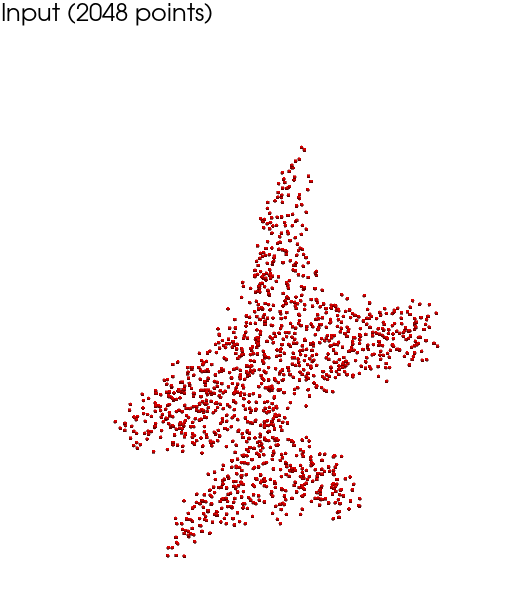
\includegraphics[width=0.6\textwidth]{figures/pointcloud/airplane/scan.png}
\caption{Projected-ShapeNet飞机样本模拟扫描位姿}
\label{fig:airplane_scan}
\end{figure}

图\ref{fig:airplane_compare}、\ref{fig:airplane_compare2}、\ref{fig:airplane_compare3}从同一视角展示了飞机样本由本算法与baseline方法的补全前后对比。左侧为输入的残缺点云（红色点云，2048个点），中间为PoinTr基线方法的补全结果（绿色点云，8192个点），右侧为本算法优化后的补全结果（蓝色点云，8192个点）。

\begin{figure}[htbp]
\centering
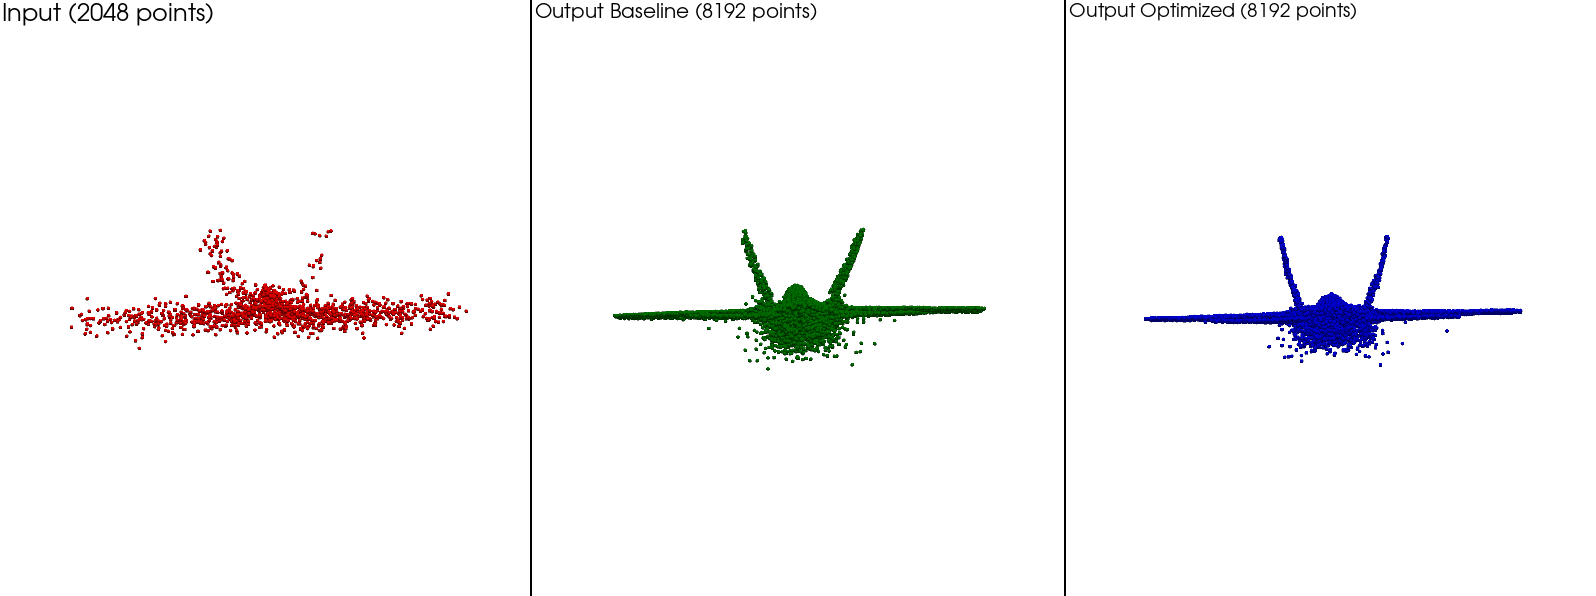
\includegraphics[width=\textwidth]{figures/pointcloud/airplane/compare-1.png}
\caption{飞机补全效果对比（视角一）}
\label{fig:airplane_compare}
\end{figure}

从图\ref{fig:airplane_compare}可以看出，在正视图视角下，PoinTr基线方法虽然能够重建出飞机的基本轮廓，但机身下方区域存在明显离群点，导致整体形状不清晰。相比之下，本算法优化后的补全结果在机身下方区域的点分布更加均匀，离群点较少，轮廓清晰，机翼与机身的过渡更加自然。

\begin{figure}[htbp]
\centering
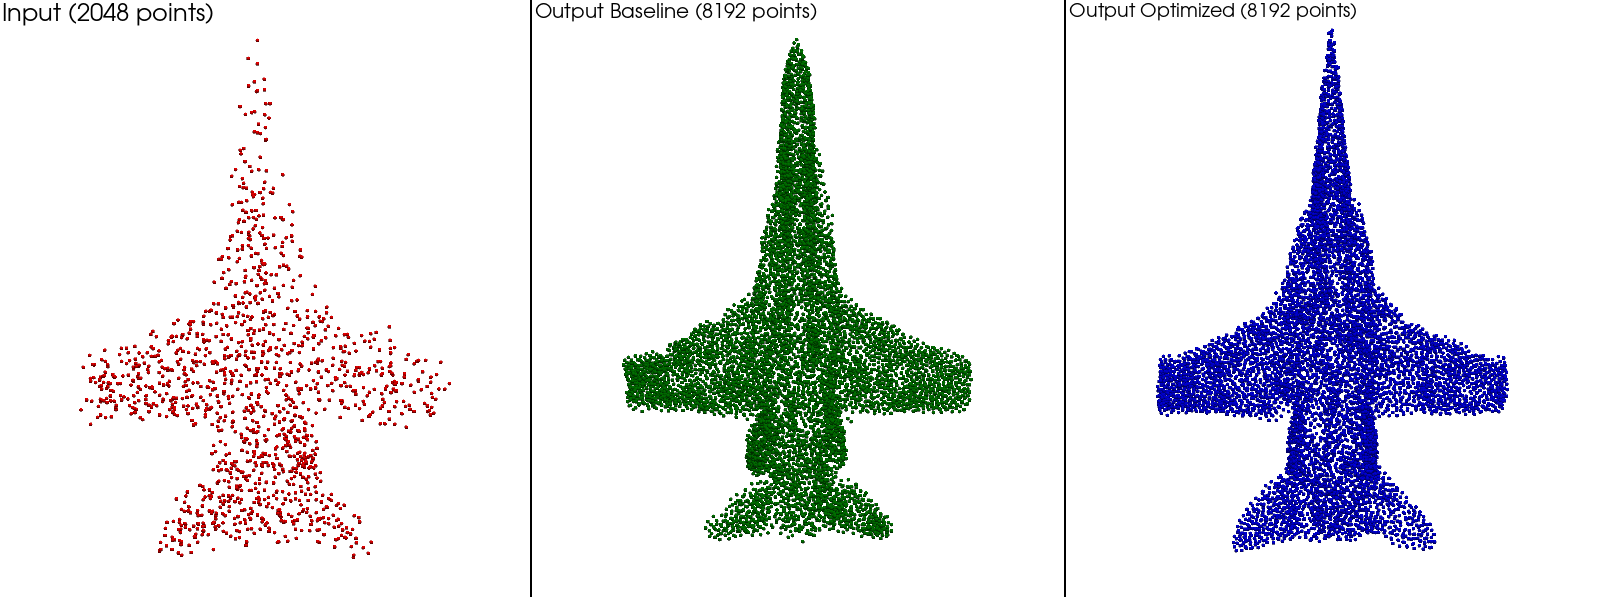
\includegraphics[width=\textwidth]{figures/pointcloud/airplane/compare-2.png}
\caption{飞机补全效果对比（视角二）}
\label{fig:airplane_compare2}
\end{figure}

图\ref{fig:airplane_compare2}从底部仰视视角展示了补全效果。在此视角下，PoinTr基线方法生成的点云在尾翼区域存在明显的原始点云缺失区域补全后局部密度不均的问题。本算法的补全结果则呈现出更加均匀的点分布，全局点密度保持一致，整体几何结构更加完整。

\begin{figure}[htbp]
\centering
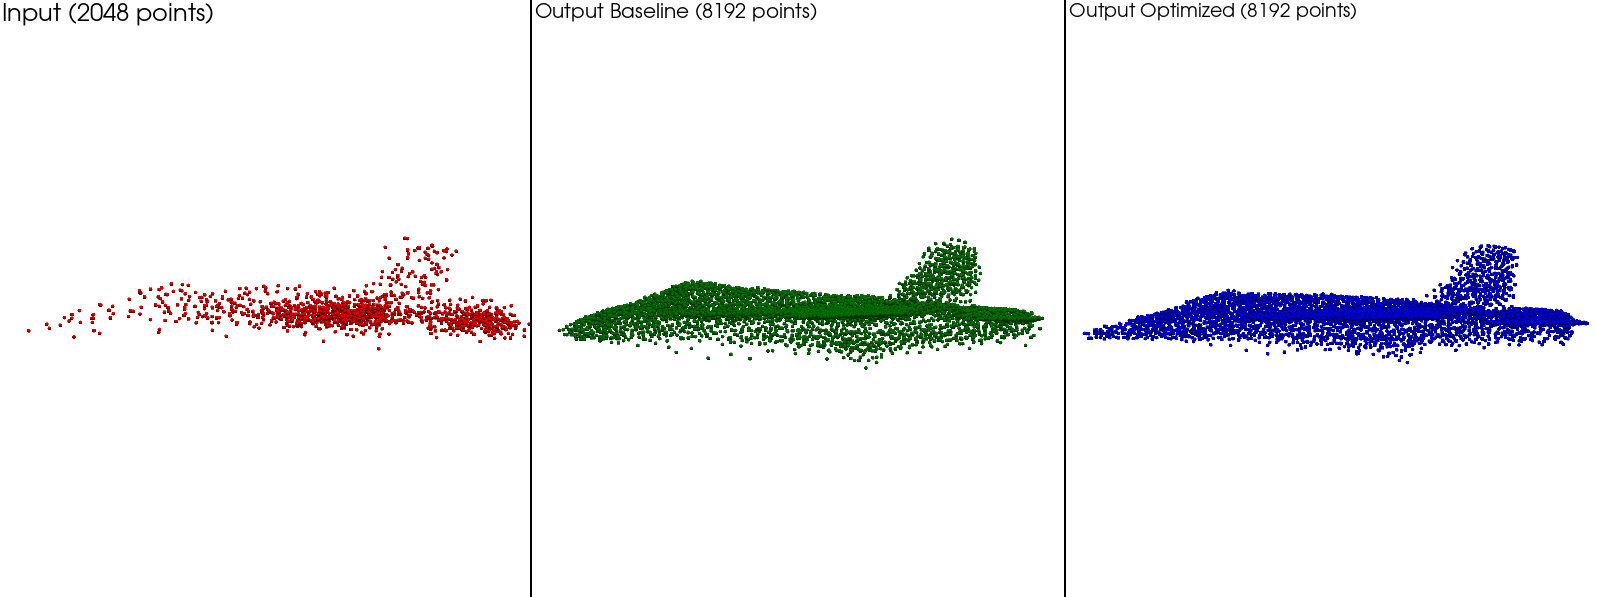
\includegraphics[width=\textwidth]{figures/pointcloud/airplane/compare-3.png}
\caption{飞机补全效果对比（视角三）}
\label{fig:airplane_compare3}
\end{figure}

图\ref{fig:airplane_compare3}从侧面视角展示了补全效果。在此视角下，PoinTr基线方法在机身腹部区域出现了严重的点云离群和密度现象。本算法通过引入DCD损失和排斥损失，有效抑制了局部点云堆积，使得机身腹部的点分布更加贴合真实表面，整体轮廓清晰，线条流畅，无明显密度不均问题。

\begin{figure}[htbp]
\centering
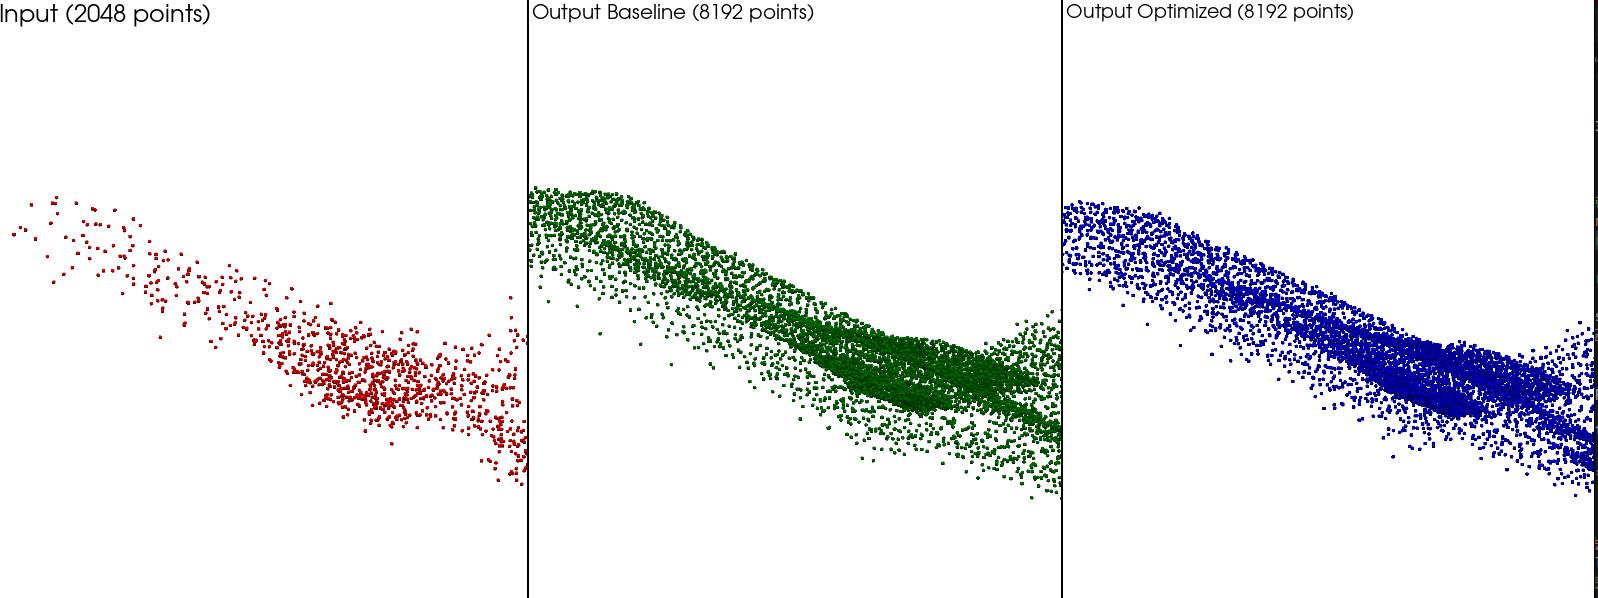
\includegraphics[width=\textwidth]{figures/pointcloud/airplane/density.png}
\caption{飞机残缺区域补全密度细节对比}
\label{fig:airplane_density}
\end{figure}

图\ref{fig:airplane_density}聚焦于飞机下防残缺区域的补全细节。从图中可以清晰地观察到，PoinTr基线方法在补全区域出现了明显的点云分层和密度不均现象，上半部分点云过度密集而需要补全的下半部分则过于洗漱。本算法的补全结果则展现出与全局密度高度一致的点分布，补全区域的点密度与原始观测区域相匹配，点云表面连续且均匀，有效验证了DCD损失和排斥损失在改善点云分布均匀性方面的作用。

(2) 吉他类别补全效果分析

图\ref{fig:guitar_scan}展示了Projected-ShapeNet数据集中吉他样本的模拟扫描位姿，本小节中Projected-ShapeNet模拟的扫描设备位于吉他上方，因此残缺点云集中在琴身区域。

\begin{figure}[htbp]
\centering
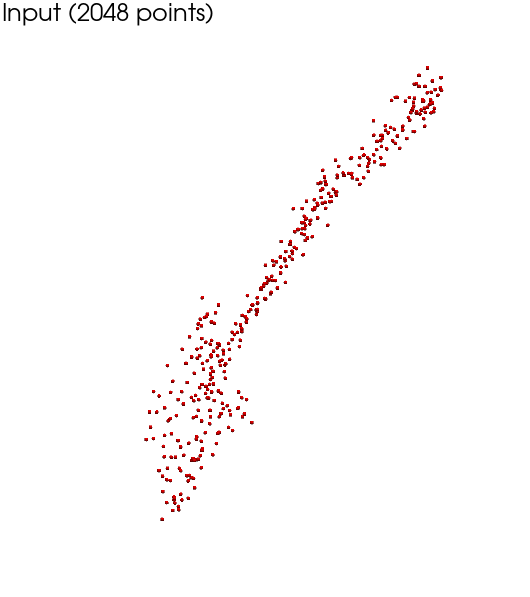
\includegraphics[width=0.6\textwidth]{figures/pointcloud/guitar/scan.png}
\caption{Projected-ShapeNet吉他样本模拟扫描位姿}
\label{fig:guitar_scan}
\end{figure}

\begin{figure}[htbp]
\centering
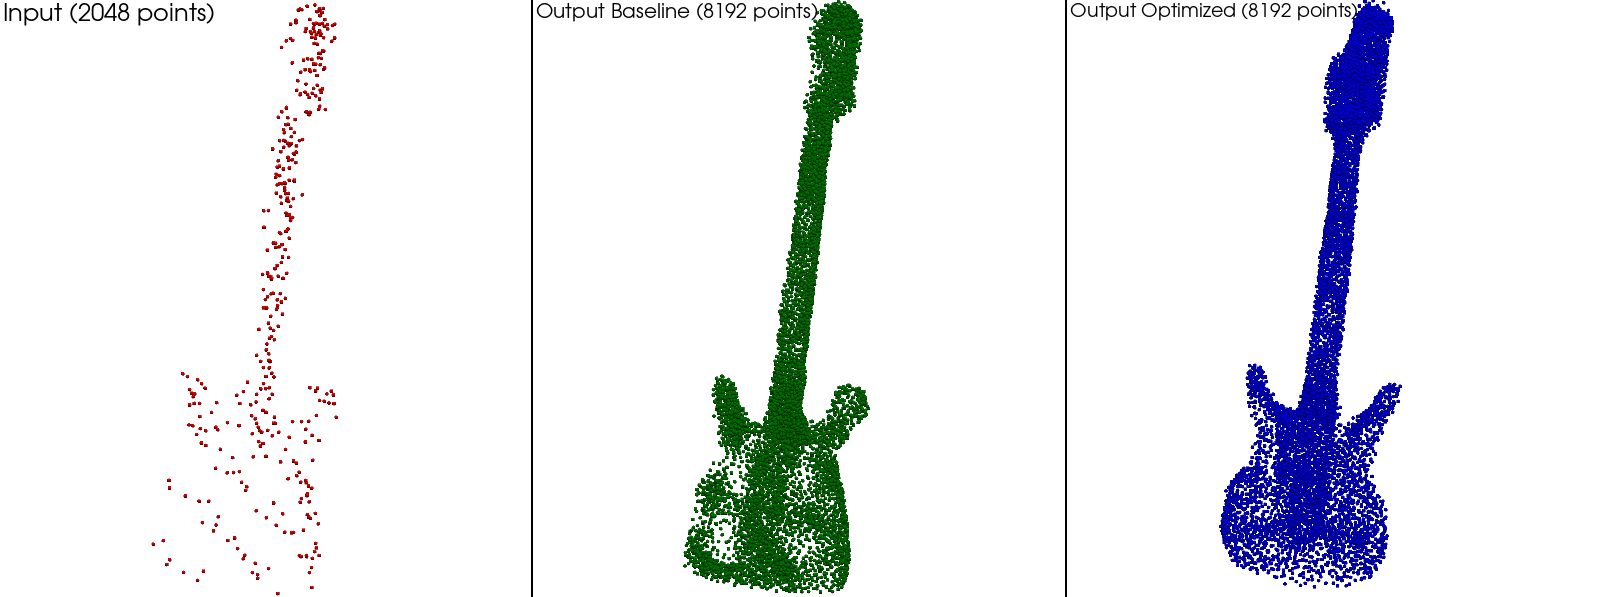
\includegraphics[width=\textwidth]{figures/pointcloud/guitar/compare-1.png}
\caption{吉他补全效果对比（视角一）}
\label{fig:guitar_compare}
\end{figure}

从图\ref{fig:guitar_compare}可以看出，在正面视角下，PoinTr基线方法虽然能够重建出吉他的基本形状，但琴身区域的点分布存在明显的不均匀现象，琴身两侧的弧形边缘处点云密度偏高，而琴身中部则相对稀疏。本算法的补全结果在琴身各区域的点密度更加均衡，琴身的弧形轮廓更加清晰，琴颈与琴身的连接处过渡更加自然。

\begin{figure}[htbp]
\centering
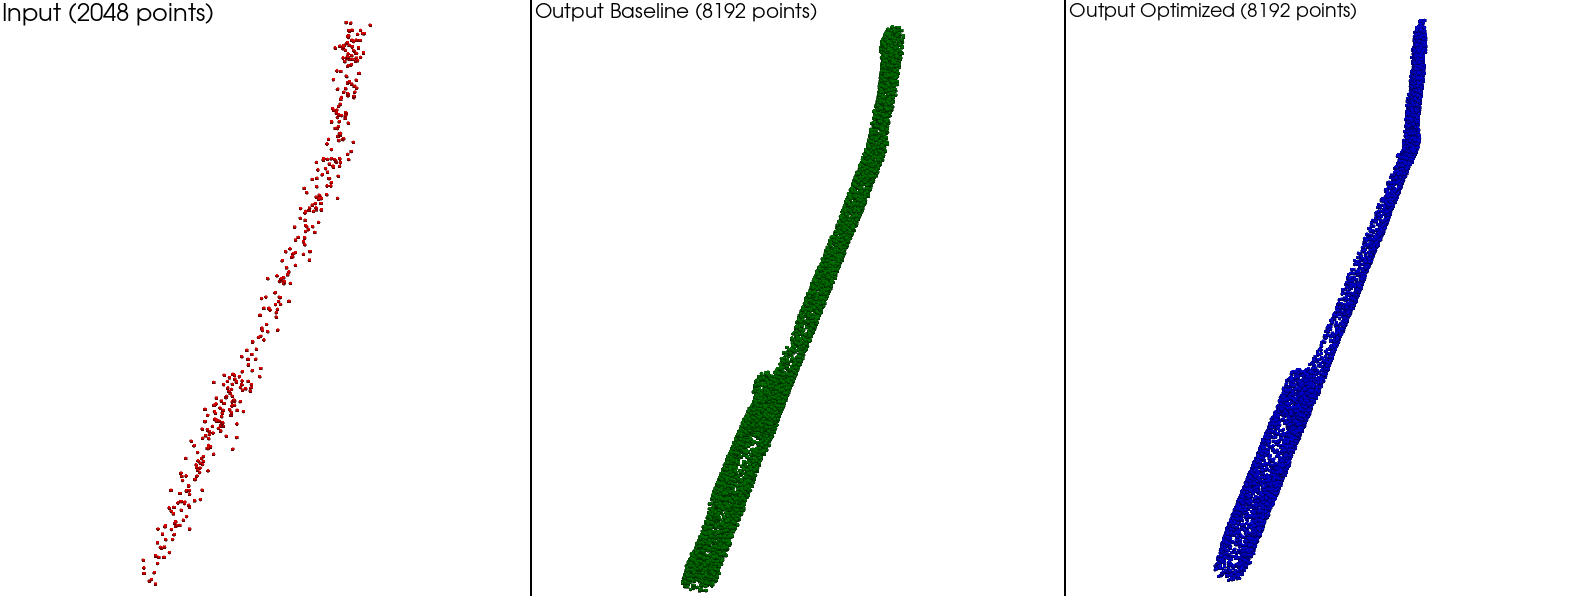
\includegraphics[width=\textwidth]{figures/pointcloud/guitar/compare-2.png}
\caption{吉他补全效果对比（视角二）}
\label{fig:guitar_compare2}
\end{figure}

图\ref{fig:guitar_compare2}从侧面视角展示了吉他琴颈的补全细节与整体轮廓。在此视角下，两个补全后的结果都没有出现明显离群点。但PoinTr基线方法生成的点云存在明显的厚度不均问题，部分区域点云过度集中导致琴颈显得过厚，而琴身与琴颈连接处过度处十分不自然，琴身也存在明显厚度不均。本算法的补全结果则呈现出均匀的琴颈厚度，轮廓清晰合理，点分布沿琴颈轴向保持一致，琴颈的几何结构更加精确。

\begin{figure}[htbp]
\centering
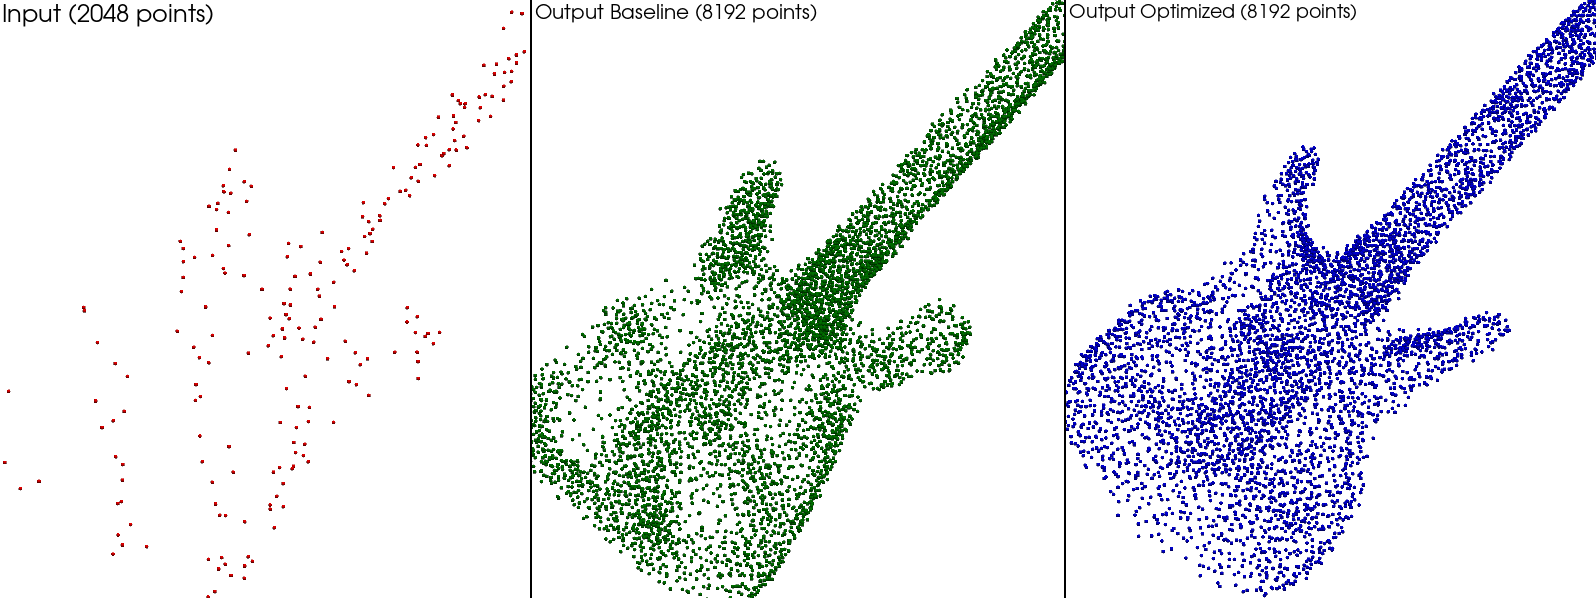
\includegraphics[width=\textwidth]{figures/pointcloud/guitar/density.png}
\caption{吉他残缺区域补全密度细节对比}
\label{fig:guitar_density}
\end{figure}

图\ref{fig:guitar_density}聚焦于吉他琴身残缺区域的补全细节。从图中可以清晰地观察到，PoinTr基线方法在琴身补全区域出现了点云密度波动现象，琴颈表面的点分布不够连续。本算法的补全结果则展现出均匀且连续的点分布，补全区域的点密度与琴身区域保持一致，琴颈表面的几何细节得到了精确还原。

(3) 可视化对比总结

综合上述可视化对比结果，本算法在点云补全效果上相较于PoinTr基线方法展现出以下优势：

（1）点云分布均匀性显著改善。通过引入DCD损失和排斥损失，本算法有效抑制了补全区域的局部点云堆积现象，使得生成点云在全局范围内保持均匀的密度分布。这一改进在飞机机身腹部、吉他琴身弧形边缘等复杂几何区域尤为明显。

（2）总体补全精度提升。本算法的补全结果在整体形状还原和局部细节精确性上均优于基线方法，补全点云与真实形状的几何偏差更小，表面连续性更好，轮廓清晰又不失细节。

（3）残缺区域补全质量提高。在结构性缺失区域，本算法能够生成与原始观测区域密度匹配的补全点云，避免了基线方法中常见的点云分层和密度波动问题，为后续的三维表面重建等下游任务提供了更高质量的输入数据。

\section{点云补全算法消融实验}

为了论证本文中优化方法的有效性，本章将使用逐步消融策略进行消融实验。与4.2.2小节相同，本章仍然采用PoinTr\cite{yu2021pointr}作为基线方法开展消融实验。

\subsection{粗粒度损失函数优化引入的影响}

PoinTr在粗粒度阶段仅使用标准CD损失进行优化，本算法在此基础上引入EMD损失，形成EMD与CD的加权组合损失。EMD通过双射匹配约束强化了骨架点云的全局拓扑对齐，而CD则保持了局部几何特征的精确性。

表\ref{tab:ablation_coarse}展示了粗粒度损失函数优化的消融实验结果。实验在ShapeNet-34数据集上进行，评价指标包括CD-L2在三种残缺程度下的表现以及F-Score@1\%。

\begin{table}[htbp]
\centering
\caption{粗粒度损失函数优化消融实验结果}
\label{tab:ablation_coarse}
\begin{tabular}{lccccc}
\toprule
\multirow{2}{*}{配置} & \multicolumn{4}{c}{CD-L2 ($\times 10^{-3}$)} & \multirow{2}{*}{F-Score@1\% ($\times 10^{-2}$)} \\
\cmidrule(lr){2-5}
& Simple & Moderate & Hard & Avg & \\
\midrule
PoinTr基线 & 0.76 & 1.05 & 1.88 & 1.23 & 42.1 \\
+ EMD损失 & 0.68 & 0.93 & 1.65 & 1.09 & 43.2 \\
\midrule
\textbf{提升幅度} & \textbf{10.5\%} & \textbf{11.4\%} & \textbf{12.2\%} & \textbf{11.4\%} & \textbf{2.6\%} \\
\bottomrule
\end{tabular}
\end{table}

从表\ref{tab:ablation_coarse}可以看出，引入EMD损失后，模型在CD-L2指标上取得了显著提升。平均CD-L2从$1.23 \times 10^{-3}$降至$1.09 \times 10^{-3}$，降幅达11.4\%。在不同残缺程度下，EMD损失的引入均带来了稳定的性能提升，其中在困难场景下的提升幅度最大（12.2\%），这表明EMD的双射匹配约束对于高缺失率情况下的全局拓扑重建具有更强的指导作用。

EMD损失的核心优势在于其对全局分布的敏感性。标准CD损失通过最近邻匹配计算预测点与真实点之间的距离，这种匹配方式允许多个预测点匹配到同一个真实点，容易导致局部点云堆积。EMD则要求建立预测点与真实点之间的一一对应关系，迫使模型在生成粗粒度点云时更加关注全局分布的均匀性。对于点云补全任务而言，粗粒度点云的全局拓扑正确性是后续细粒度优化的基础，EMD损失的引入为模型提供了更强的全局约束，使得生成的骨架点云更加接近真实形状的整体轮廓。

此外，EMD损失的引入也带来了F-Score@1\%指标的提升，从42.1\%增至43.2\%。这表明粗粒度点云质量的改善不仅体现在CD指标上，也反映在生成点云与真实点云的局部匹配精度上。高质量的粗粒度点云为后续的细粒度优化提供了更好的起点，使得模型能够在正确的全局结构基础上进行局部细节的完善。

\subsection{自适应查询生成机制影响分析}

在粗粒度损失函数优化的基础上，本实验进一步引入自适应查询生成机制。该机制包含两个关键组件：自适应查询排序和去噪任务辅助训练。自适应查询排序通过学习性重要性评估来优化查询点的选择，优先选择几何特征丰富区域的点作为查询；去噪任务辅助训练则通过在训练过程中引入额外的去噪目标来增强模型的鲁棒性和泛化能力。

表\ref{tab:ablation_query}展示了自适应查询生成机制的消融实验结果。

\begin{table}[htbp]
\centering
\caption{自适应查询生成机制消融实验结果}
\label{tab:ablation_query}
\begin{tabular}{lccccc}
\toprule
\multirow{2}{*}{配置} & \multicolumn{4}{c}{CD-L2 ($\times 10^{-3}$)} & \multirow{2}{*}{F-Score@1\% ($\times 10^{-2}$)} \\
\cmidrule(lr){2-5}
& Simple & Moderate & Hard & Avg & \\
\midrule
+ EMD损失 & 0.68 & 0.93 & 1.65 & 1.09 & 43.2 \\
+ 查询排序 & 0.61 & 0.84 & 1.48 & 0.98 & 44.1 \\
+ 去噪任务 & 0.57 & 0.78 & 1.38 & 0.91 & 44.7 \\
\midrule
\textbf{总提升幅度} & \textbf{16.2\%} & \textbf{16.1\%} & \textbf{16.4\%} & \textbf{16.5\%} & \textbf{3.5\%} \\
\bottomrule
\end{tabular}
\end{table}

从表\ref{tab:ablation_query}可以看出，自适应查询生成机制的两个组件均对模型性能产生了积极影响。引入查询排序后，平均CD-L2从$1.09 \times 10^{-3}$降至$0.98 \times 10^{-3}$，降幅达10.1\%。查询排序机制通过学习性重要性评估，使得模型能够自动识别几何特征丰富的关键区域，并将有限的查询点资源分配给最具信息量的位置。这种自适应的查询点选择策略相比于固定的FPS采样，能够更好地适应不同物体的几何复杂度分布，从而提升整体补全质量。

在查询排序的基础上进一步引入去噪任务后，平均CD-L2继续降至$0.91 \times 10^{-3}$，额外降幅为7.1\%。去噪任务的引入为模型提供了额外的监督信号，使得模型不仅需要学习如何从部分观测推断完整形状，还需要学习如何从带噪声的输入中恢复准确的几何位置。这种多任务学习策略增强了模型对输入扰动的容忍度，提升了在未见数据上的泛化性能。

自适应查询排序和去噪任务辅助训练之间存在协同效应。查询排序确保了查询点的质量，使得解码器能够基于最具信息量的查询点进行细粒度生成；去噪任务则通过额外的监督信号增强了模型对查询点特征的利用效率。两者的结合使得模型在CD-L2指标上累计提升了16.5\%，F-Score@1\%从43.2\%增至44.7\%。

\subsection{细粒度损失函数优化引入的影响}

在前两项优化的基础上，本实验最后引入细粒度损失函数优化。PoinTr在细粒度阶段仅使用标准CD损失进行优化，本算法在此基础上引入DCD损失和排斥损失，形成多损失协同优化的策略。DCD通过密度感知权重防止多个预测点匹配到同一个真实点，排斥损失则通过惩罚过近的点对来促使点云均匀分布。

表\ref{tab:ablation_fine}展示了细粒度损失函数优化的消融实验结果。

\begin{table}[htbp]
\centering
\caption{细粒度损失函数优化消融实验结果}
\label{tab:ablation_fine}
\begin{tabular}{lccccc}
\toprule
\multirow{2}{*}{配置} & \multicolumn{4}{c}{CD-L2 ($\times 10^{-3}$)} & \multirow{2}{*}{F-Score@1\% ($\times 10^{-2}$)} \\
\cmidrule(lr){2-5}
& Simple & Moderate & Hard & Avg & \\
\midrule
+ 自适应查询生成机制 & 0.57 & 0.78 & 1.38 & 0.91 & 44.7 \\
+ DCD损失\&排斥损失 & 0.51 & 0.67 & 1.19 & 0.79 & 45.5 \\
\midrule
\textbf{总提升幅度} & \textbf{10.5\%} & \textbf{14.1\%} & \textbf{13.8\%} & \textbf{13.2\%} & \textbf{1.8\%} \\
\bottomrule
\end{tabular}
\end{table}

从表\ref{tab:ablation_fine}可以看出，细粒度损失函数优化的两个组件均对模型性能产生了显著影响。引入DCD损失与排斥损失后，平均CD-L2降至$0.79 \times 10^{-3}$，降幅达13.2\%。DCD通过密度感知权重机制，有效识别和惩罚那些导致局部点云堆积的预测结果，促使生成的点云更加均匀地分布在真实点云的表面。与标准CD相比，DCD对局部密度变化更加敏感，能够更好地捕捉细粒度点云的分布质量。而排斥损失的作用机制类似于物理系统中的排斥力，当两个点之间的距离小于某个阈值时，会产生一个排斥力将它们推开，从而避免点的过度聚集。排斥损失与DCD损失的协同作用使得细粒度点云在全局结构正确的基础上，具备了更加均匀和自然的点分布特性。两者综合极大提升了模型的密度感知能力，针对原始点云残缺区域的补全密度失衡的痛点问题进行了针对性解决。

综合三项优化措施，本算法相较于PoinTr基线在CD-L2指标上累计提升了35.8\%（从$1.23 \times 10^{-3}$降至$0.79 \times 10^{-3}$），F-Score@1\%提升了8.1\%（从42.1\%增至45.5\%）。表\ref{tab:ablation_summary}汇总了完整的消融实验结果。

\begin{table}[htbp]
\centering
\caption{完整消融实验结果汇总}
\label{tab:ablation_summary}
\begin{tabular}{lccccc}
\toprule
\multirow{2}{*}{配置} & \multicolumn{4}{c}{CD-L2 ($\times 10^{-3}$)} & \multirow{2}{*}{F-Score@1\% ($\times 10^{-2}$)} \\
\cmidrule(lr){2-5}
& Simple & Moderate & Hard & Avg & \\
\midrule
PoinTr基线 & 0.76 & 1.05 & 1.88 & 1.23 & 42.1 \\
+ 粗粒度损失优化 & 0.68 & 0.93 & 1.65 & 1.09 & 43.2 \\
+ 自适应查询生成机制 & 0.57 & 0.78 & 1.38 & 0.91 & 44.7 \\
+ 细粒度损失优化 & 0.51 & 0.67 & 1.19 & 0.79 & 45.5 \\
\midrule
\textbf{总提升幅度} & \textbf{32.9\%} & \textbf{36.2\%} & \textbf{36.7\%} & \textbf{35.8\%} & \textbf{8.1\%} \\
\bottomrule
\end{tabular}
\end{table}

从表\ref{tab:ablation_summary}可以看出，三项优化措施基本独立且互补，共同推动了模型性能的提升。粗粒度损失优化主要改善了全局拓扑结构的正确性，为后续优化奠定了良好的基础；自适应查询生成机制提升了查询点的质量和模型对查询点特征的利用效率；细粒度损失优化则进一步改善了生成点云的分布均匀性和局部细节质量。三者的协同作用使得本算法在ShapeNet-34数据集上取得了显著优于PoinTr基线的补全性能。

\section{三维表面重建算法结果展示与分析}

点云补全作为三维视觉领域的基础任务，其最终目的是为下游应用提供高质量的三维几何数据。为了验证本算法优化后的补全点云在实际应用中的价值，本节将补全结果输入第三章所述的泊松表面重建流程，生成三角网格模型，并从可视化角度分析补全算法优化对三维表面重建效果的积极影响。

(1) 飞机类别重建结果分析

图\ref{fig:reconstruct_airplane_front}和图\ref{fig:reconstruct_airplane_back}分别展示了基于PoinTr基线补全点云和本算法优化补全点云重建的飞机网格模型的正面和背面视图。

\begin{figure}[htbp]
\centering
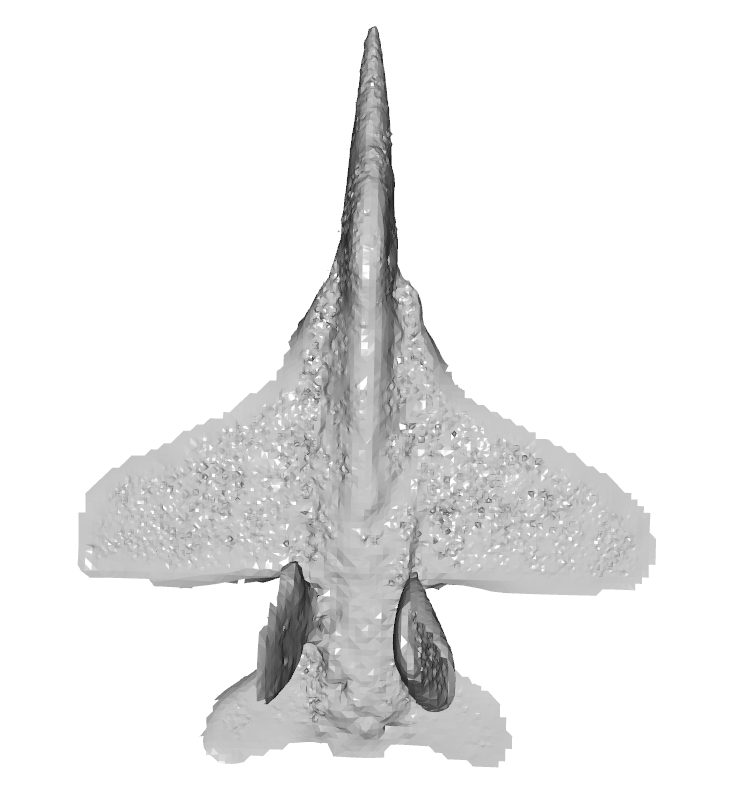
\includegraphics[width=0.45\textwidth]{figures/reconstruct/airplane/baseline-front.png}
\hfill
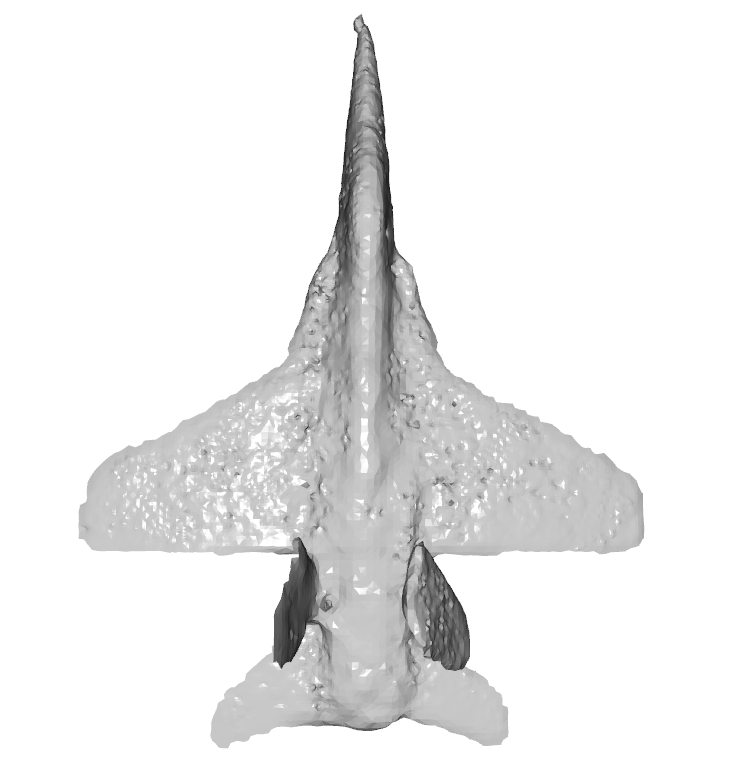
\includegraphics[width=0.45\textwidth]{figures/reconstruct/airplane/optimized-front.png}
\caption{飞机网格重建结果俯视视图对比（左：PoinTr基线，右：本算法优化）}
\label{fig:reconstruct_airplane_front}
\end{figure}

\begin{figure}[htbp]
\centering
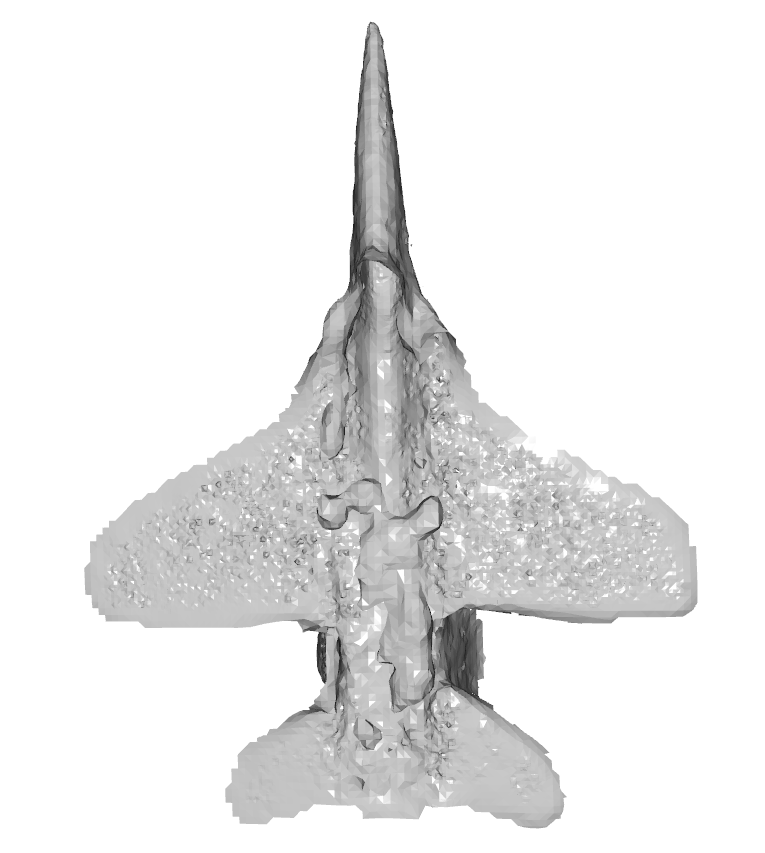
\includegraphics[width=0.45\textwidth]{figures/reconstruct/airplane/baseline-back.png}
\hfill
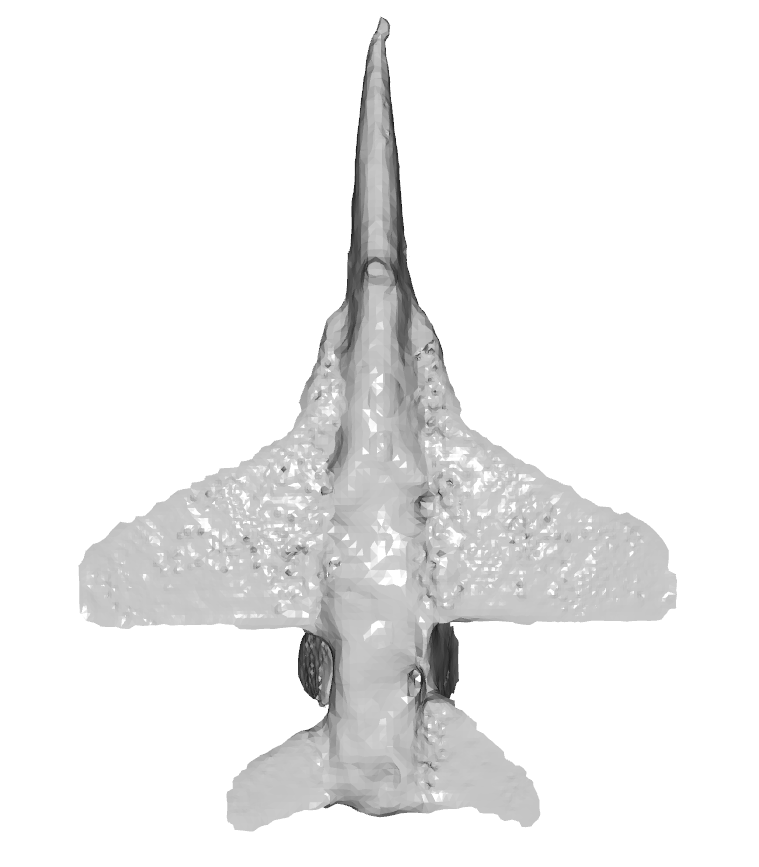
\includegraphics[width=0.45\textwidth]{figures/reconstruct/airplane/optimized-back.png}
\caption{飞机网格重建结果仰视视图对比（左：PoinTr基线，右：本算法优化）}
\label{fig:reconstruct_airplane_back}
\end{figure}

从正面视图对比可以看出，基于PoinTr基线补全点云重建的网格模型在机身背部区域存在明显的表面粗糙和局部凹陷现象。这是由于基线方法在补全过程中产生的点云堆积和密度不均导致泊松重建算法在该区域生成了不规则的三角面片，进而形成网格表面的凹凸不平。相比之下，基于本算法优化补全点云重建的网格模型在机身腹部区域呈现出光滑连续的表面，原有的凹陷和粗糙区域得到了有效修复。这一改善直接归因于本算法引入的损失函数优化对点云分布均匀性的改善，使得补全区域的点密度与全局保持一致，为泊松重建提供了更加可靠的输入数据。

从背面视图对比可以进一步观察到，基线方法重建的网格在机翼与机身连接处存在明显的边界模糊和表面断裂现象，机身腹部更是几乎完全被空洞占据。这是由于基线补全点云在该区域的轮廓不够清晰，点分布存在局部稀疏和空洞，导致法线估计不准确，进而影响泊松重建的质量。本算法优化后的补全点云在机翼与机身连接处具有更加清晰的轮廓和均匀的点分布，使得重建网格在该区域的表面连续性显著提升，机翼的几何结构得到了更加精确的还原。

(2) 吉他类别重建结果分析

图\ref{fig:reconstruct_guitar_front}和图\ref{fig:reconstruct_guitar_back}分别展示了基于PoinTr基线补全点云和本算法优化补全点云重建的吉他网格模型的正面和背面视图。

\begin{figure}[htbp]
\centering
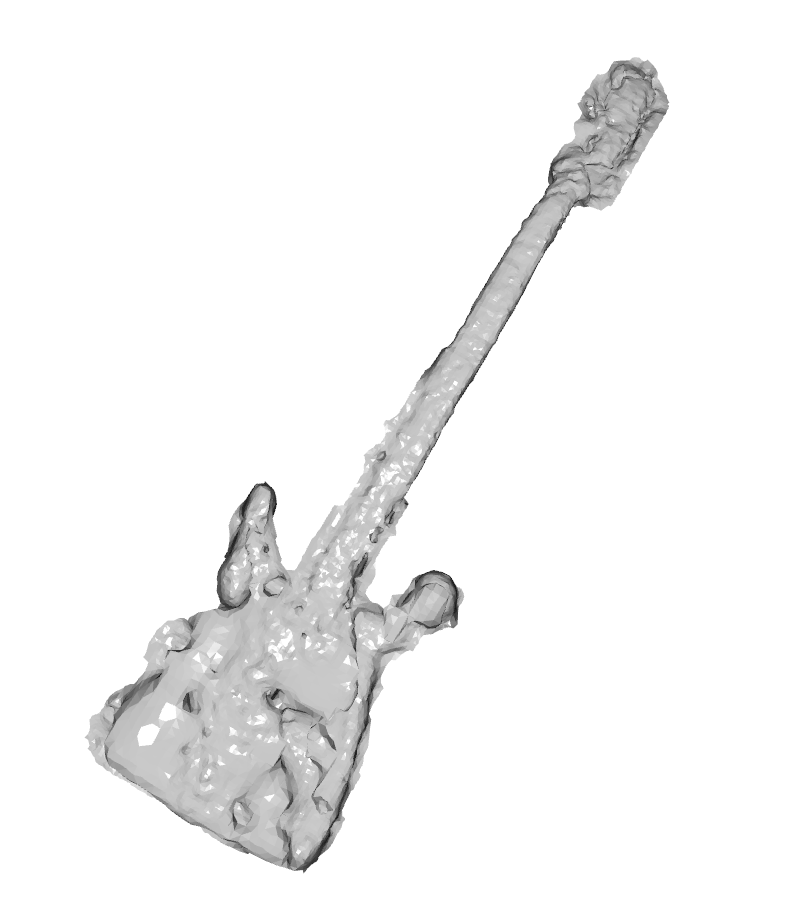
\includegraphics[width=0.45\textwidth]{figures/reconstruct/guitar/baseline-front.png}
\hfill
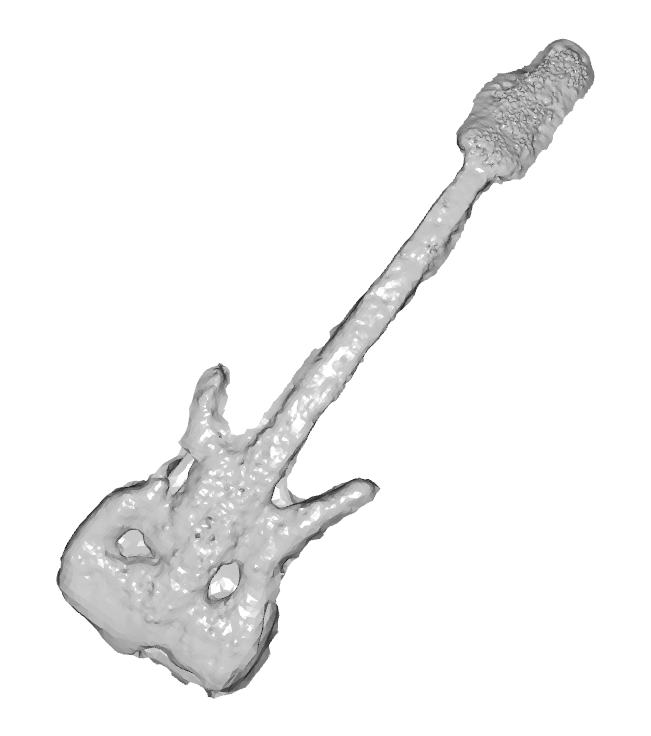
\includegraphics[width=0.45\textwidth]{figures/reconstruct/guitar/optimized-front.png}
\caption{吉他网格重建结果正面视图对比（左：PoinTr基线，右：本算法优化）}
\label{fig:reconstruct_guitar_front}
\end{figure}

\begin{figure}[htbp]
\centering
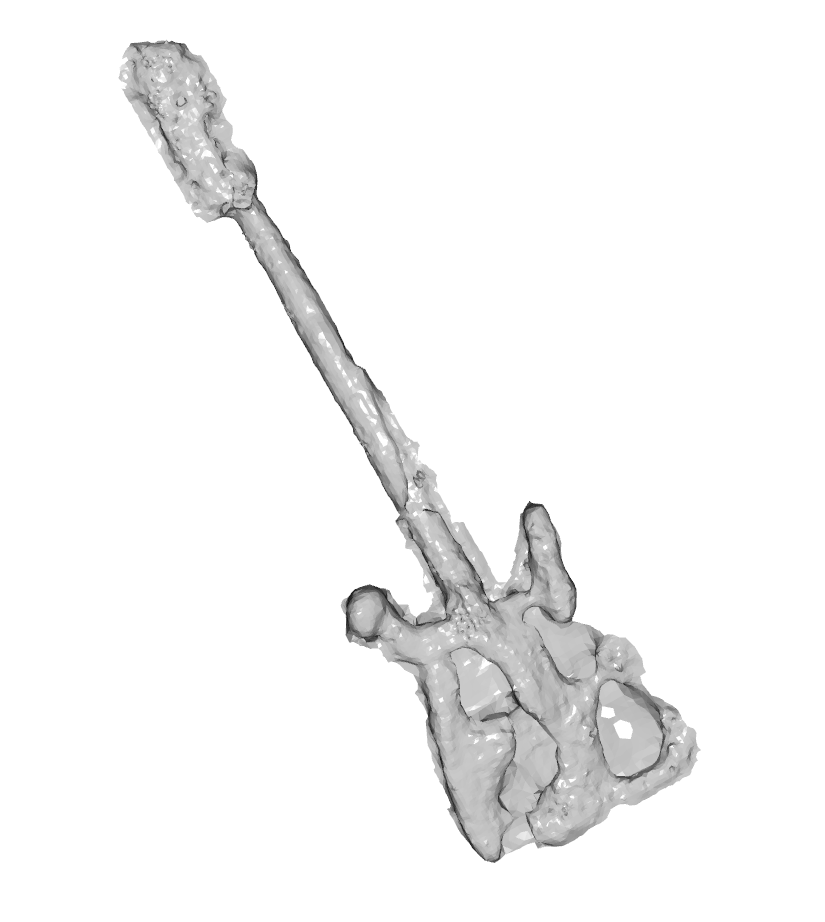
\includegraphics[width=0.45\textwidth]{figures/reconstruct/guitar/baseline-back.png}
\hfill
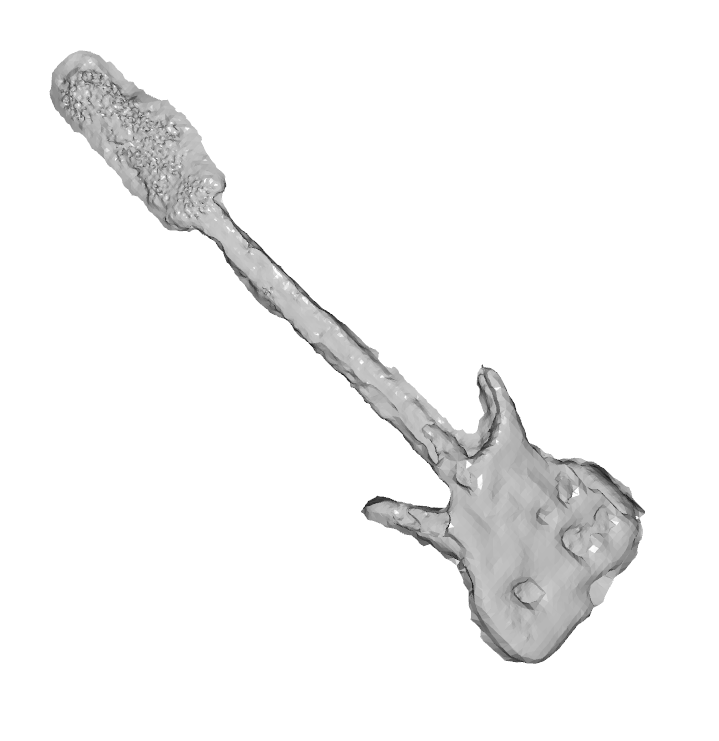
\includegraphics[width=0.45\textwidth]{figures/reconstruct/guitar/optimized-back.png}
\caption{吉他网格重建结果背面视图对比（左：PoinTr基线，右：本算法优化）}
\label{fig:reconstruct_guitar_back}
\end{figure}

从正面视图对比可以看出，基于PoinTr基线补全点云重建的吉他网格模型在琴身弧形边缘处存在明显的表面锯齿和局部变形。这是由于基线方法在补全琴身弧形区域时产生的点云密度波动，导致泊松重建算法在该区域生成了不规则的三角面片分布。相比之下，基于本算法优化补全点云重建的吉他网格模型在琴身各区域的表面更加光滑，弧形边缘的轮廓更加清晰，琴身的整体几何形状得到了更加精确的还原。

从背面视图对比可以观察到，基线方法重建的网格在琴颈区域存在明显的表面不连续和局部空洞现象。这是由于基线补全点云在琴颈区域的点分布不够均匀，部分区域点云过于密集而另一些区域则出现稀疏，导致法线估计和泊松重建在该区域的质量下降。本算法优化后的补全点云在琴颈区域呈现出均匀且连续的点分布，使得重建网格在该区域的表面质量显著提升，琴颈的几何结构得到了更加精确的还原。

(3) 重建结果综合分析

综合上述重建结果对比，本算法优化后的补全点云为三维表面重建带来了以下积极影响：

（1）轮廓清晰度提升。本算法通过自适应查询生成机制和混合损失函数优化，使得补全点云在物体边缘和结构转折处的轮廓更加清晰。清晰的点云轮廓为法线估计提供了更加准确的局部几何信息，进而提升了泊松重建的表面质量。

（2）点云分布均匀性改善。本算法引入的损失函数优化有效抑制了补全区域的局部点云堆积和空洞现象，使得生成点云在全局范围内保持均匀的密度分布。均匀的点分布为泊松重建提供了更加可靠的输入数据，减少了重建过程中因点密度波动导致的表面粗糙和局部变形。

（3）整体精度提升。本算法优化后的补全点云在整体形状还原和局部细节精确性上均优于基线方法，使得重建网格模型在几何精度和表面质量上均得到了显著提升。这一改善在飞机机身腹部、吉他琴身弧形边缘等复杂几何区域尤为明显。

上述结果表明，点云补全算法的优化不仅体现在补全点云本身的定量指标提升上，更能够直接转化为下游三维表面重建任务的质量改善。本算法通过系统性的损失函数优化和查询生成机制改进，有效解决了补全区域点云密度失衡的核心问题，为三维视觉领域的实际应用提供了更加可靠的技术支撑。

\section{本章小结}

本章通过系统的实验验证了本文基于Transformer的点云补全算法的卓越性能。在ShapeNet-34数据集上的对比实验表明，本算法在CD-L2和F-Score@1\%指标上均取得了具有竞争力的结果，优于PoinTr、SnowflakeNet等经典方法。在Projected-ShapeNet数据集上的可视化对比进一步验证了本算法在点云分布均匀性和整体补全精度上的优势。消融实验结果表明，粗粒度损失优化、自适应查询生成机制和细粒度损失优化三项措施累计使CD-L2指标降低35.8\%，F-Score@1\%提升8.1\%，各项优化措施独立且互补，共同推动了模型性能的提升。三维表面重建结果展示表明，本算法优化后的补全点云能够有效改善下游重建任务的质量，在轮廓清晰度、点云分布均匀性和整体精度方面均带来积极影响，为点云补全算法的实际应用提供了有力支撑。
% !Mode:: "TeX:UTF-8"
\chapter{总结与展望}
\label{cha:summary}

\section{研究工作总结}

本文围绕点云补全任务中的核心问题展开研究，针对残缺点云补全过程中出现的密度失衡与分布不均匀问题，提出了一套基于Transformer的点云补全算法优化方案，并构建了从补全点云到三维网格模型的完整表面重建流程。本文的主要研究工作与贡献总结如下：

（1）提出了基于混合损失函数的点云补全优化策略。在粗粒度生成阶段，引入EMD（Earth Mover's Distance）损失替代单一的标准CD损失，通过双射匹配约束强化了骨架点云的全局拓扑对齐能力。在细粒度优化阶段，设计了包含密度感知倒角距离（DCD）和排斥损失的混合损失函数，通过密度感知权重机制和局部排斥力约束，有效改善了生成点云的分布均匀性。分阶段权重调度策略使得模型能够在不同训练阶段获得最合适的优化目标，实现了多损失之间的协同优化。

（2）引入了自适应查询生成机制。通过自适应查询排序和去噪任务辅助训练两个组件，提升了查询点的质量和模型对查询点特征的利用效率。查询排序机制通过学习性重要性评估，使得模型能够自动识别几何特征丰富的关键区域；去噪任务则通过额外的监督信号增强了模型对输入扰动的容忍度，提升了泛化性能。

（3）构建了完整的三维表面重建流程。基于泊松表面重建算法，实现了从补全点云到三角网格模型的转换。该流程涵盖法线估计与定向、泊松重建、密度阈值过滤和Taubin平滑等关键步骤，能够基于补全后的高质量点云生成表面连续、细节丰富的三维网格模型，为点云补全算法的实际应用提供了有效的下游任务验证。

（4）通过系统的实验验证了算法的有效性。在ShapeNet-34数据集上的对比实验表明，本算法在CD-L2和F-Score@1\%指标上均取得了具有竞争力的结果，优于PoinTr、SnowflakeNet、SeedFormer等经典方法。消融实验进一步验证了各项优化措施的独立贡献，三项优化措施累计使CD-L2指标降低35.8\%（从$1.23 \times 10^{-3}$降至$0.79 \times 10^{-3}$），F-Sore@1\%提升8.1\%（从42.1\%增至45.5\%）。实验结果充分证明了本文所提优化策略的有效性和合理性。

\section{未来研究展望}

尽管本文在点云补全算法优化方面取得了一定的研究成果，但受限于研究时间和实验条件，仍存在若干值得进一步探索的方向：

（1）架构层面的进一步优化。从对比实验结果可以看出，本算法与当前SOTA级模型（如AnchorFormer、PCD-MT等）仍存在一定的性能差距。未来工作可以考虑在架构设计方面引入创新性机制，例如探索Mamba等新型状态空间模型与Transformer的融合，或者设计更加高效的特征聚合策略，以进一步提升补全精度和计算效率。

（2）面向复杂场景的泛化能力提升。本文的实验评估主要基于ShapeNet-34和Projected-ShapeNet数据集，这些数据集的残缺模式相对规则。未来工作可以在更加复杂和真实的残缺场景下验证算法的鲁棒性，例如处理由真实深度相机采集的点云数据，或者应对极端遮挡、严重噪声等挑战性条件。此外，探索跨类别的零样本补全能力也是一个有价值的研究方向。

（3）下游应用的拓展。点云补全作为三维视觉领域的基础任务，其下游应用涵盖三维重建、机器人抓取、自动驾驶、虚拟现实等多个方向。未来工作可以针对特定的应用场景，探索点云补全算法与下游任务的联合优化策略，实现端到端的性能提升。例如，在机器人抓取任务中，补全质量直接影响抓取姿态的估计精度；在自动驾驶场景中，补全算法可以帮助构建更加完整的环境三维表示。
% \include{contents/chap06}
% \include{contents/conclusion}
\bibliography{reference/refs}

\backmatter
% \begin{appendix}
% \chapter{学校模板提示（附录部分）}

暂无
% \end{appendix}

% 致谢
\begin{acknowledgement}

行文至此，我的本科学习生涯也即将落下帷幕。回望四年时光，从初入校园的懵懂到如今的逐渐成熟，每一步成长都离不开师长的教诲、亲友的陪伴与母校的栽培。在此，谨向所有在我求学路上给予帮助与支持的人致以最诚挚的谢意。

首先，诚挚感谢我的导师张景峤老师。从选题立意到论文撰写，张老师始终给予我悉心的指导与耐心的帮助。每当我在研究中遇到瓶颈，老师总能以渊博的学识和丰富的经验为我指点迷津，帮助我理清思路、突破难关。老师严谨求实的治学态度、精益求精的工作作风，让我受益匪浅，也将成为我未来人生道路上的宝贵财富。

其次，深深感谢我的家人与挚友。家人的理解与包容是我勇往直前的最大动力，无论顺境逆境，他们始终默默支持着我的每一个选择。同窗好友们在学业上的切磋探讨、生活中的关心鼓励，为这段求学岁月增添了无数温暖与欢乐。能与你们同行，是我莫大的幸运。

最后，衷心感谢上海大学计算机工程与科学学院。四年来，学院完善的培养体系、优质的教学资源和浓厚的学术氛围，为我提供了广阔的成长平台。在这里，我不仅学到了扎实的专业知识，更培养了独立思考与探索创新的能力。母校的栽培之恩，我将永远铭记于心。

纸短情长，难尽谢忱。愿所有关心帮助过我的人平安顺遂，愿我们都能在各自的道路上砥砺前行、不负韶华。

\rightline{张嘉翊}
\rightline{上海大学宝山校区}
\rightline{2026 年 XX 月 XX 日}

\end{acknowledgement}



\includepdf[pages={1}]{back-cover.pdf}

\end{document}
